\section{Liquid Argon Time Projection Chamber}
\label{sec:tpc-all}

The MicroBooNE \lartpc drifts and collects charge to produce fine-grained images of the ionization that is liberated by charged particles traversing a volume of highly-purified liquid argon.  This section describes the design and implementation of the \lartpc in the experiment.

The \lartpc is composed of three major structures: the cathode, the field cage, and the anode. A negative voltage is introduced via a feedthrough passing through nozzle N2 on the cryostat and applied at the cathode, which defines an equipotential surface.   A uniform electric field between the cathode and the anode planes is established by a series of field rings connected by a voltage divider chain starting at the cathode and ending at the anode plane.   Facing the cathode planes are the sense wire planes: two induction planes (referred to as the ``U'' and ``V'' planes) with wires oriented at $\pm60^{\circ}$ from vertical, followed by one collection plane (referred to as the ``Y'' plane) with vertically-oriented wires.   The wires of the anode planes are the sensing elements that detect the ionization created by charged particles traveling through the LArTPC.  Figure \ref{fig:tpc-cryostat} depicts the assembled MicroBooNE \lartpc after insertion into the cryostat, showing details of the cathode, field cage, and anode plane.  Table \ref{tab:tpcparam} lists the main parameters of the MicroBooNE LArTPC, which will be described in detail in this section.  

%Opposite the cathode, and oriented parallel to it are the sense wire planes which are maintained at a potential close to ground.  


\begin{table}[!htb]
   \centering
     \caption{MicroBooNE \lartpc design parameters and nominal operating conditions.} 
    \begin{tabular}{lr} % Column formatting, @{} suppresses leading/trailing space
    \hline
    Parameter & Value \\
    \hline
    %\lartpc (active) dimensions ($h\times w\times l$) & 2.325 m $\times$ 2.560 m $\times$ 10.368 m\\
    %\lartpc (active) mass & 90 tons\\
   % \hline
    $\#$ Anode planes & 3\\
     Anode planes spacing& 3 mm \\
     Wire pitch & 3 mm  \\
     Wire type & SS, diam. 150 $\mu$m\\
     Wire coating & 2$\mu$m Cu, 0.1$\mu$m Ag\\
     Design Wire tension & 6.9N $\pm$ 1.0N\\
     $\#$ wires (total) & 8256 \\
     $\#$ Induction0 plane (U) wires & 2400 \\
     $\#$ Induction1 plane (V) wires & 2400 \\
     $\#$ Collection plane (Y) wires & 3456 \\
     Wire orientation (w.r.t. vertical) & +60$^{\circ}$,-60$^{\circ}$,0$^{\circ}$ (U,V,Y) \\
     \hline
     Cathode voltage (nominal) & -128 kV \\
     Bias voltages (U,V,Y) & -200 V, 0 V, +440 V \\
     Drift-field & 500 V/cm\\
   %  U-V gap field & 666.7 V/cm \\
    % V-Y gap field & 1466.7 V/cm \\
     Max. Drift Time, Cathode to U (at 500 V/cm) & 1.6 ms\\
    \hline
    $\#$ Field-cage steps & 64\\
    Ring-to-ring voltage step & 2.0 kV\\
    \hline
   \end{tabular}
   \label{tab:tpcparam}
\end{table} 


\begin{figure}
\centering	
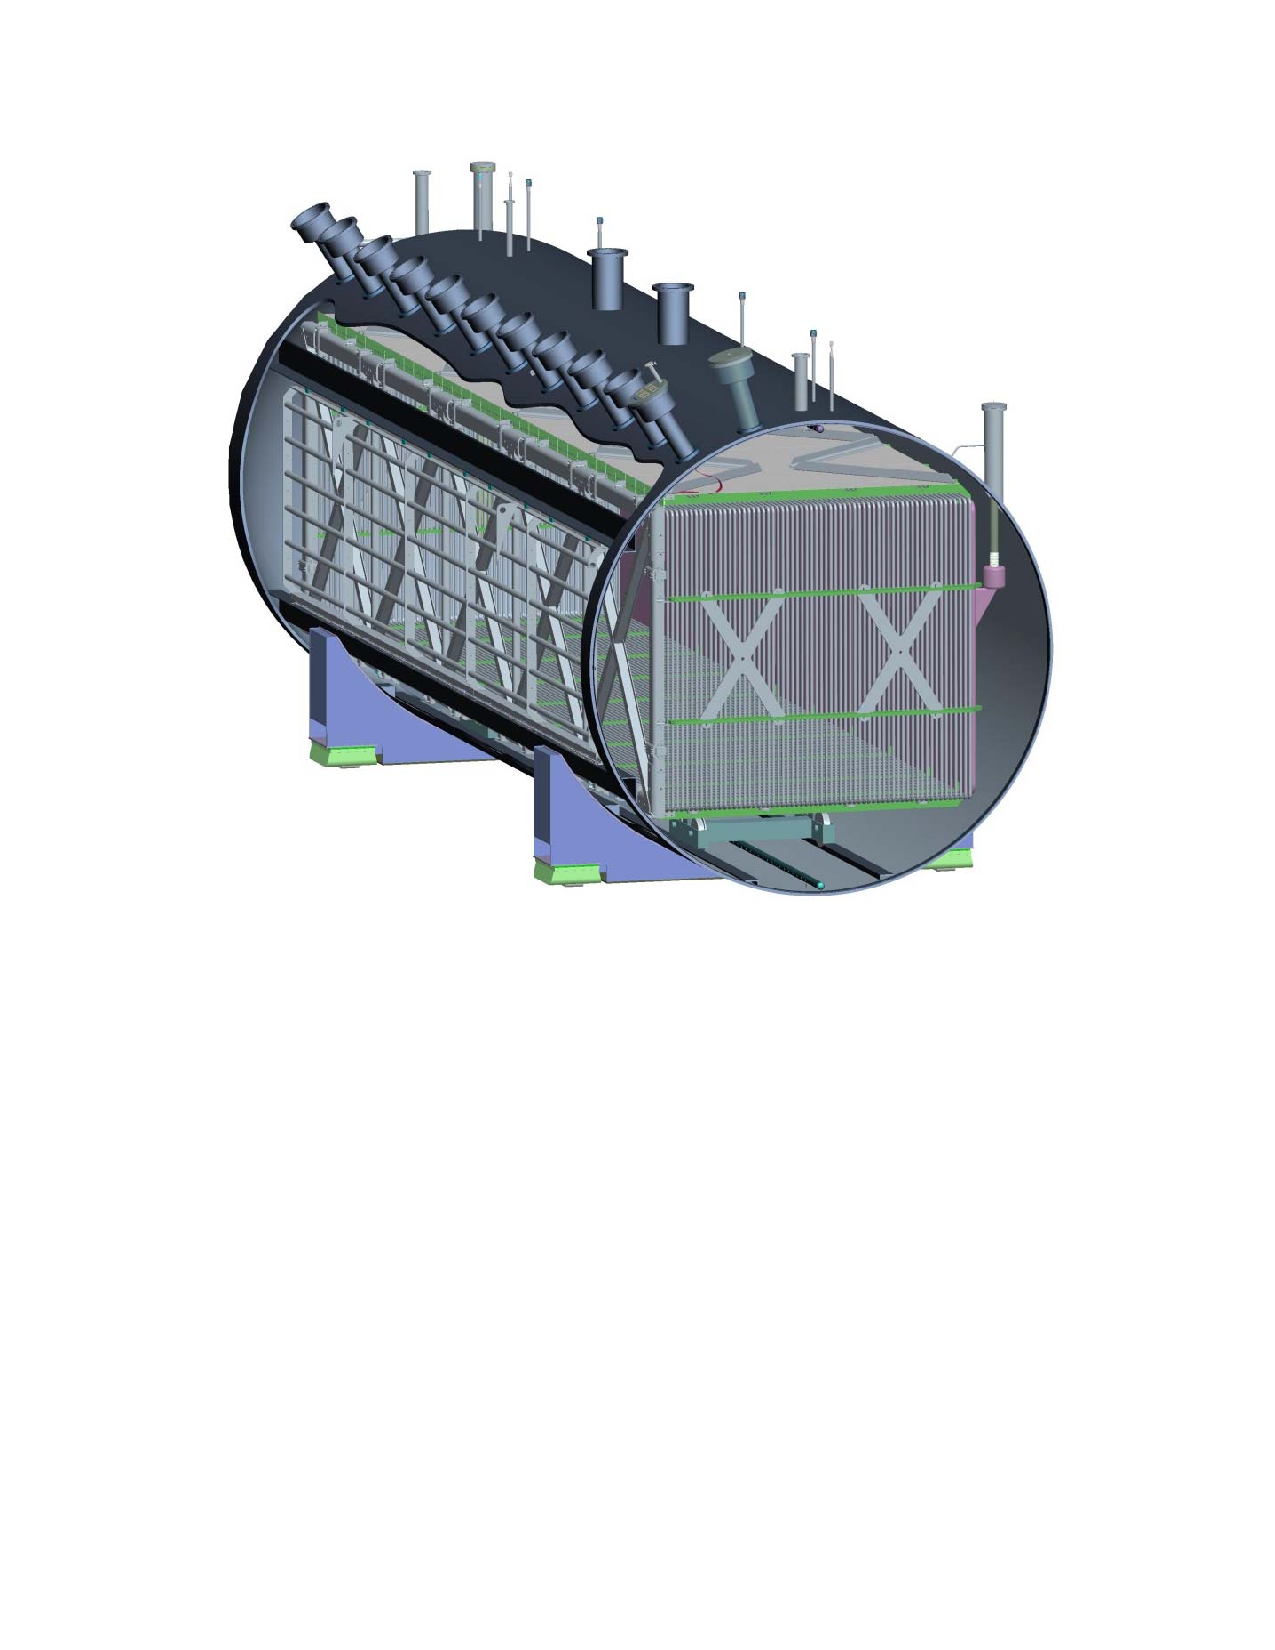
\includegraphics[width=0.8\linewidth]{figures/cryo_tpc.pdf}
\caption{Schematic diagram of the MicroBooNE \lartpc, depicted as it is arranged inside the cryostat.}
\label{fig:tpc-cryostat}
\end{figure}


%\input{tpc-mechanical}
\subsection{Cathode}
%{\it{(Jen, (Bo?))}}
The cathode is assembled from 9 individual stainless steel sheets (Type 304, 2.3 mm thick) that are fastened to a supporting frame by hex-head stainless-steel button screws. The outer edge of the cathode frame consists of round stainless steel tubes of 5.08 cm outer diameter and 3.18 mm wall thickness.  Within this outer edge, square tubes with 5.08 cm $\times$ 5.08 cm cross-sectional area, and 3.18 mm wall thickness, are fastened together with button head screws, forming a support structure upon which the cathode sheets are attached.  The individual components of the support structure are further welded together to eliminate sharp features from this high-potential surface.  The exterior frame and support structure of the cathode, and also an interior view, are shown in figure~\ref{fig:tpc-cathode}. The cathode plane sheets are shimmed according to survey data to make the cathode as flat and as parallel to the anode frame as possible, resulting in the two surfaces being parallel to within 0.0413$^{\circ}$.  Flatness of the cathode is evaluated relative to a best fit plane of survey data (more than 10000 survey points recorded with a laser tracker). The largest deviations of the cathode from the best fit plane are +6.6 mm and -6.5 mm. Approximately 55$\%$ of the measured survey points fall within +/-3 mm of the best fit plane, and more than 90$\%$ of the points fall within $\pm$5 mm.  Figure~\ref{fig:tpc-cathode-survey} shows the results of the survey, with deviations from flat represented as color-coded data extending away from the nominal plane of an ideal cathode. %%Source: Jonathan's SBND DocDB #437

\begin{figure}
\centering	
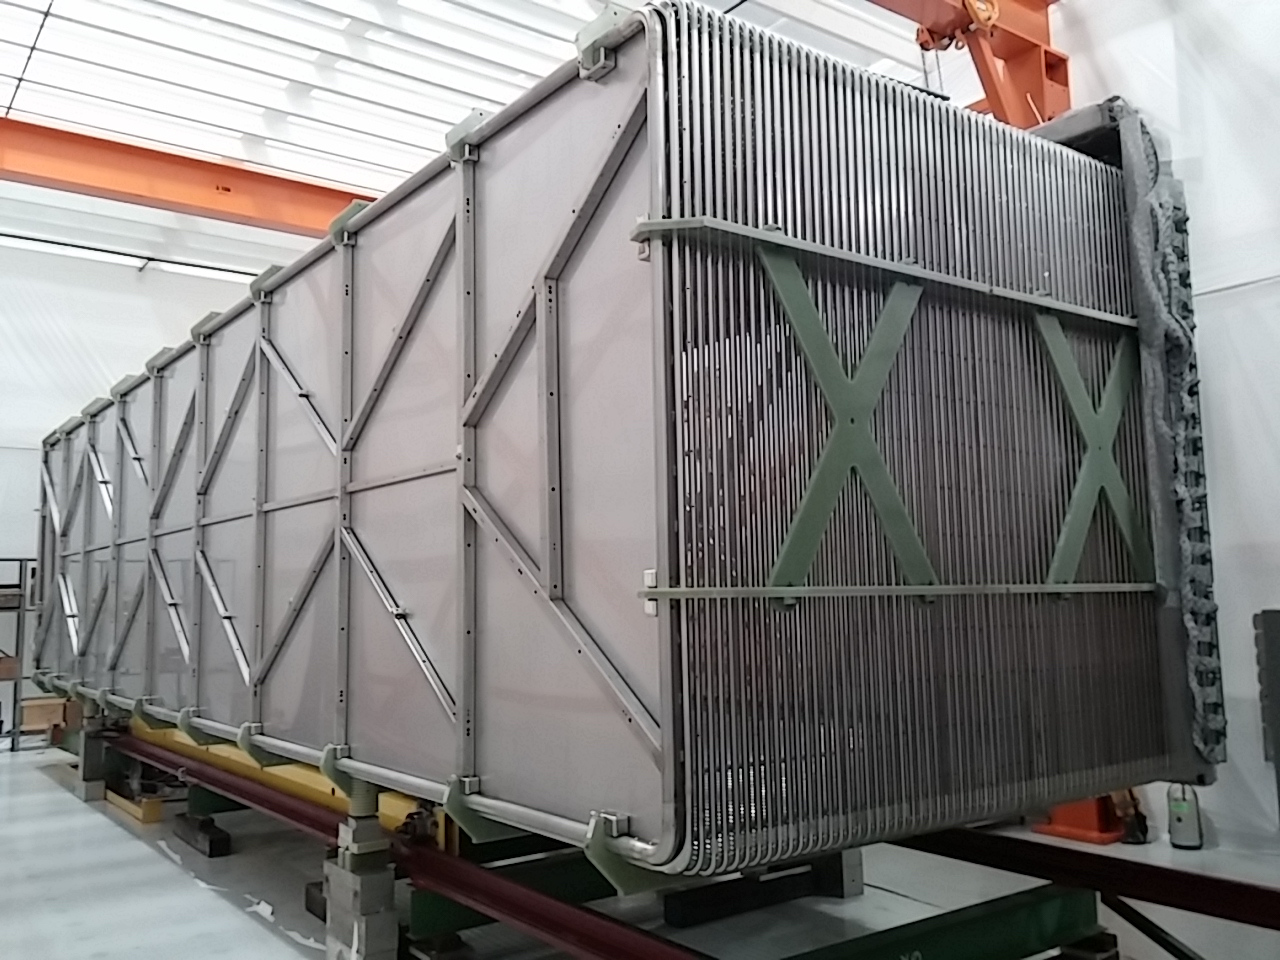
\includegraphics[width=0.62\linewidth]{figures/tpc-completed-upstream-left.jpg}
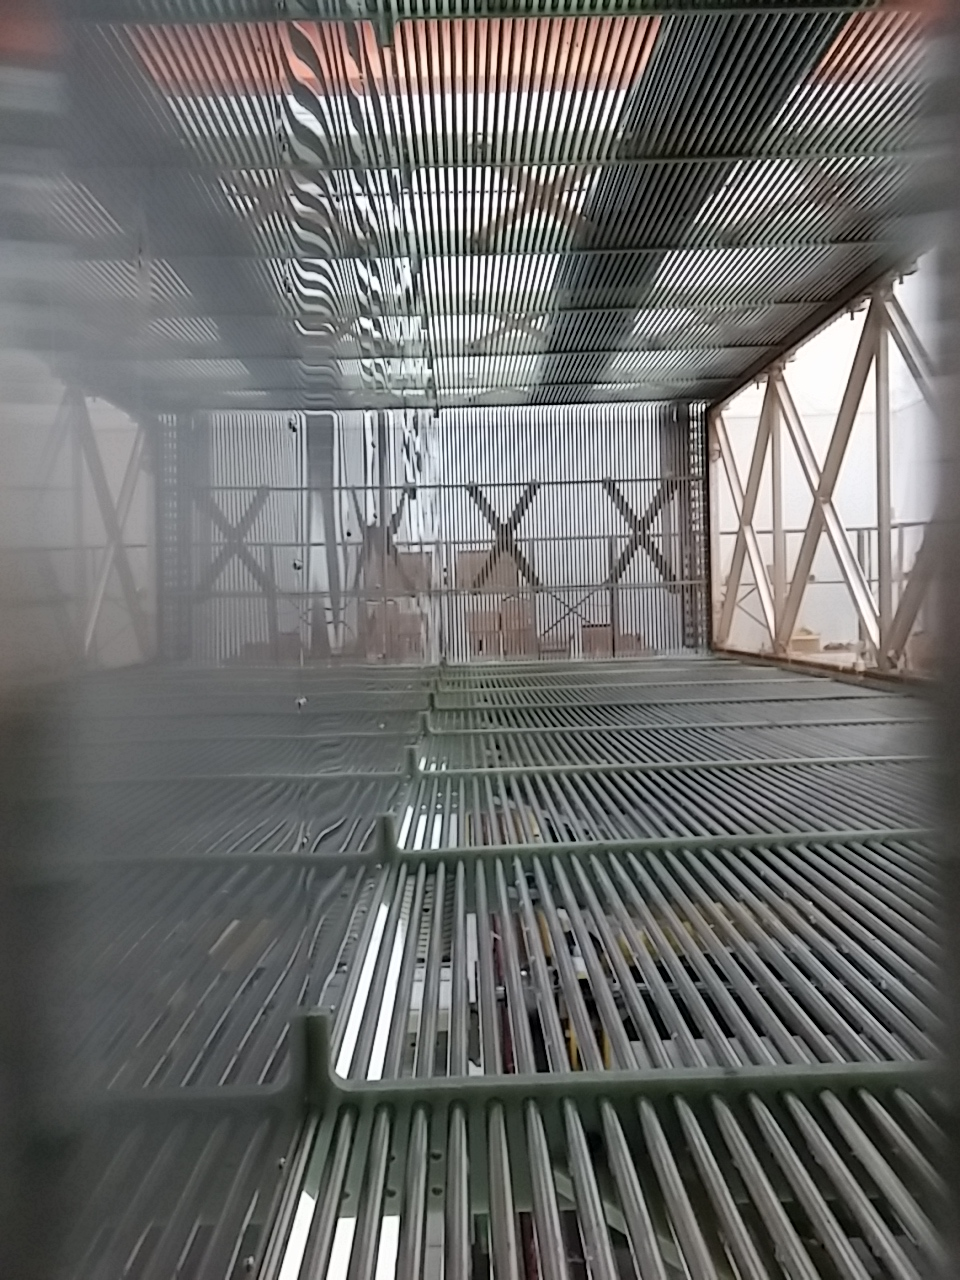
\includegraphics[width=0.62\linewidth]{figures/tpc-upstream-interior.jpg}
\caption{Top: Exterior view showing the cathode frame and structural supports to which cathode sheets are fastened.  Bottom: Interior view of cathode plane as viewed from the upstream end of the \lartpc, showing cathode sheets.  Note that the cathode sheets are polished, so a reflection is is clearly present in this photograph.}
\label{fig:tpc-cathode}
\end{figure}

%\begin{figure}[htb]
%\centering	
%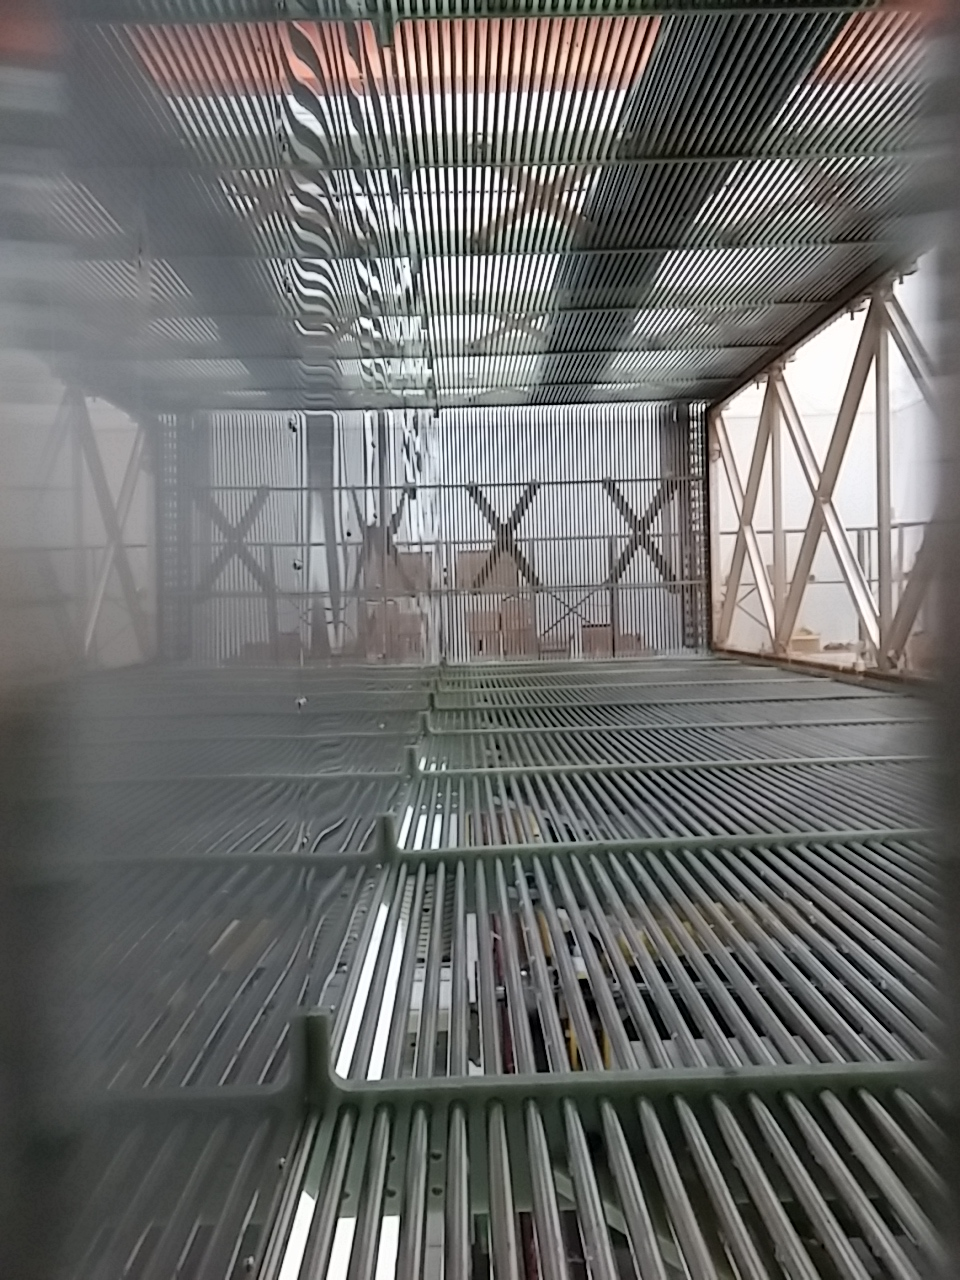
\includegraphics[width=0.55\linewidth]{figures/tpc-upstream-interior.jpg}
%\caption{Interior view of cathode plane as viewed from the upstream end of the \lartpc, showing cathode sheets.}
%\label{fig:tpc-cathode-interior}
%\end{figure}

\begin{figure}
\centering
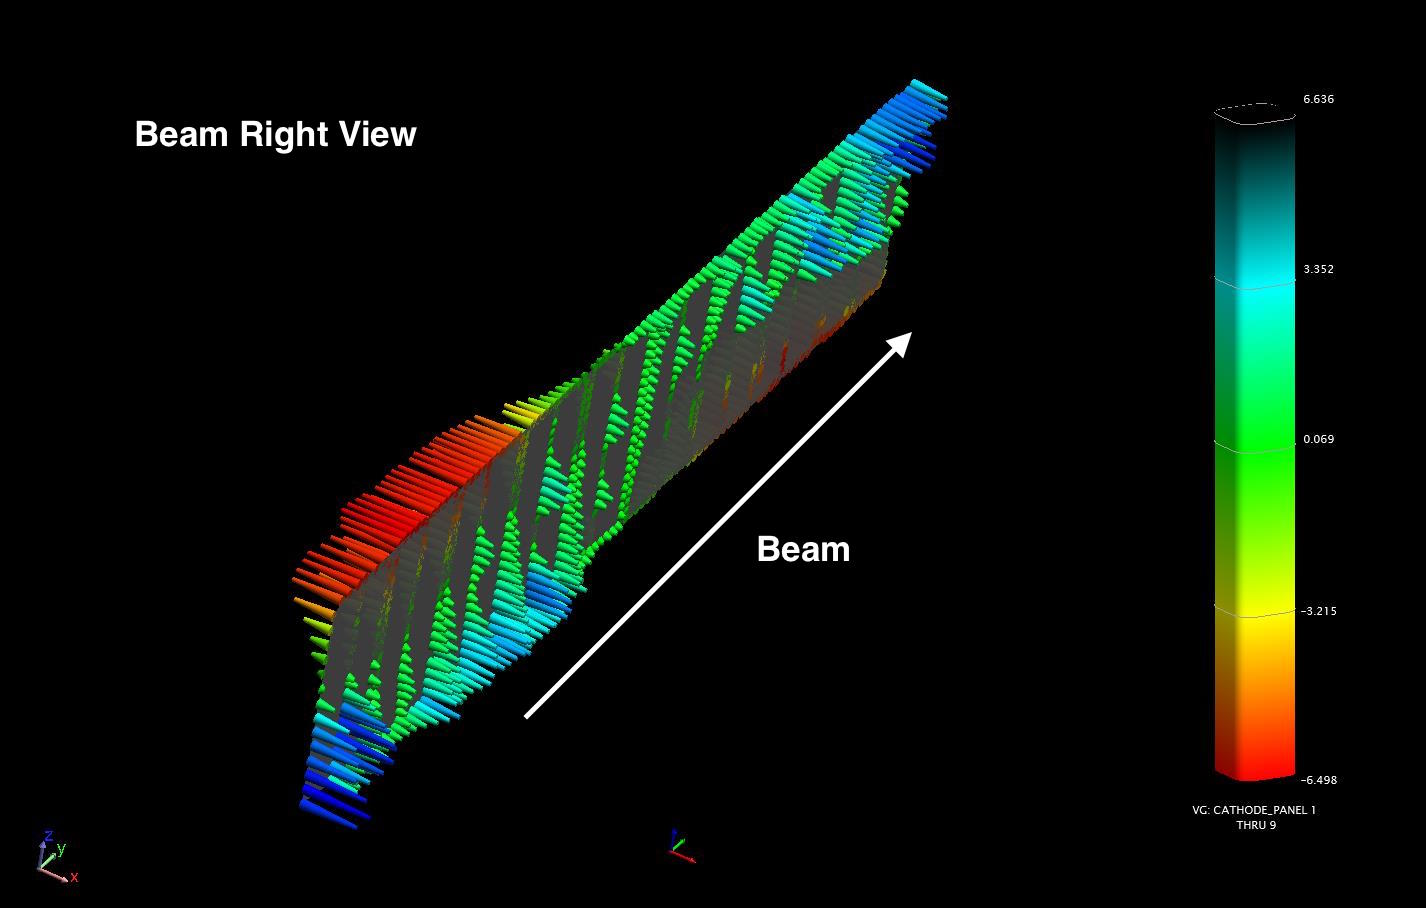
\includegraphics[width=0.75\linewidth]{figures/Cathode_BeamRight.jpg}
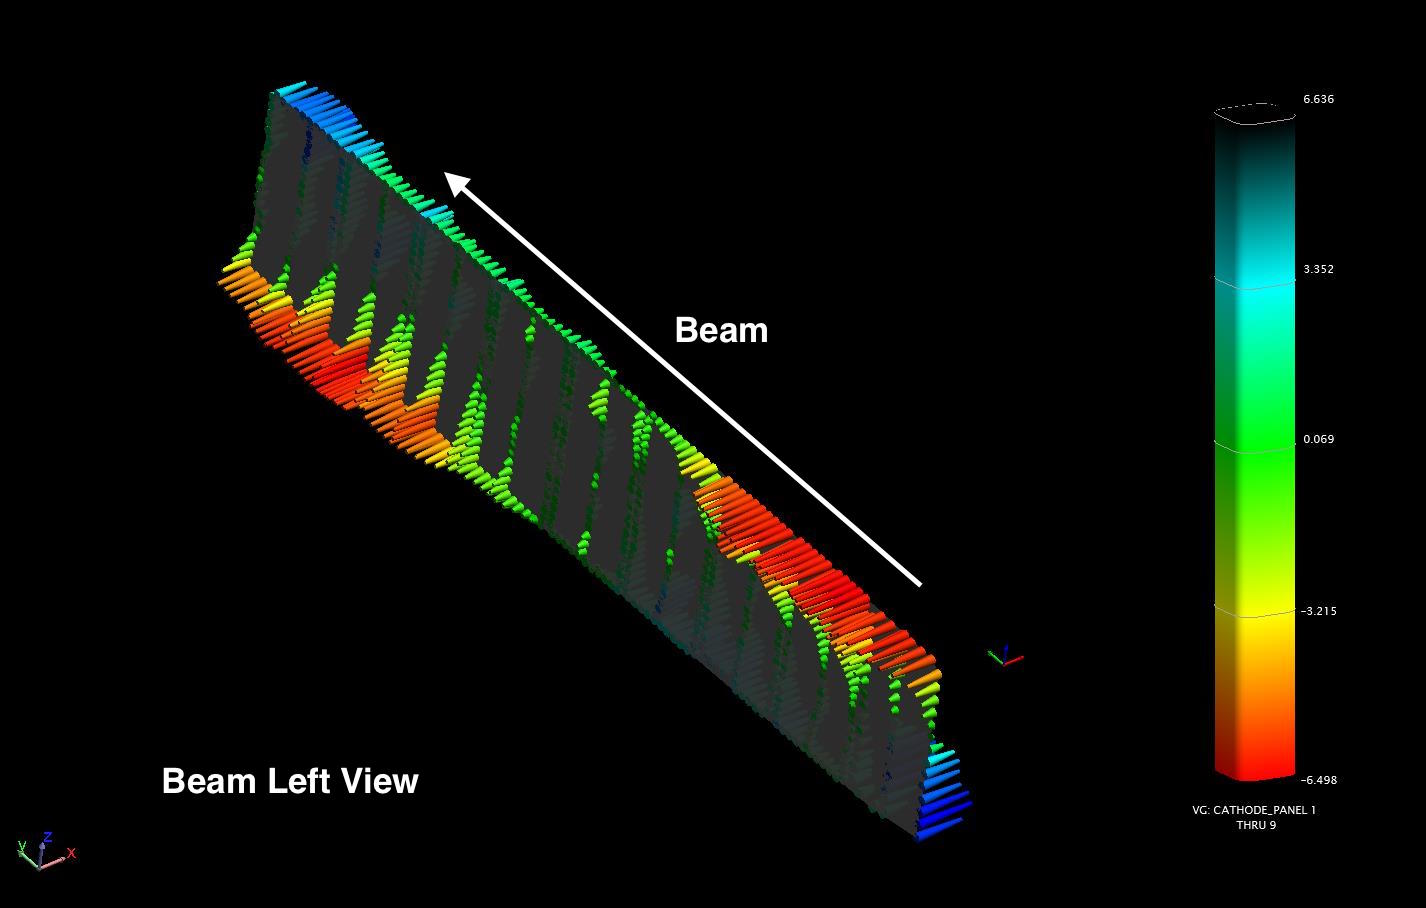
\includegraphics[width=0.75\linewidth]{figures/Cathode_BeamLeft.jpg}
\caption{Survey results showing the flatness of the cathode, as viewed from the interior (top) and exterior (bottom) sides, after shimming.  Color scale extends from -6.498 mm (red) to +6.636 mm (blue).}
\label{fig:tpc-cathode-survey}
\end{figure}

\subsection{Field Cage}
%{\it{Anne, Jen}}
The field cage encloses the volume between the cathode plane and the anode wire planes, and creates a region with a uniform electric field.  The volume defined by the interior of the field cage, bounded by the anode and cathode planes, is referred to as the ``active'' volume.   The field cage structure consists of 64 individual sets of thin-walled stainless steel tubes (2.54 cm OD, 0.51 mm wall thickness), each shaped into a rectangular loop framing the perimeter of the active volume. These 64 loops are mounted parallel to the cathode and anode planes, as shown in figure~\ref{fig:tpc-cathode}, and are held in place by a G-10 rib support structure. Each field cage loop is electrically connected to its neighbors via a resistor divider chain (described in following section), causing each loop to operate at a different electrical potential, which in turn maintains a uniform electric field between the cathode and anode planes. For a nominal -128~kV cathode voltage, the difference in potential between adjacent field cage loops is 2~kV, ramping down the total potential in equidistant steps from cathode to anode. The distance from center-to-center of adjacent field cage loops is 4.0~cm.

Each field cage loop is assembled from 2.07 m long vertical pipes on the upstream and downstream ends of the \lartpc, and on the top and bottom from two 5.18 m long horizontal pipes connected by a stainless steel coupling in the center.  Each tube has venting holes approximately every 15 cm to allow for effective purging from atmosphere and avoid any trapped volumes.  

The four corners of each field cage loop are curved with a radius of 5.24 cm. Each corner is formed by three parts: two couplings and an elbow, shown in figure~\ref{fig:tpc-fieldcage-elbows}. The couplings make the connections between the pipes and the elbow. The thin-walled tubes and elbows slip-fit over the ends of the couplings with a 2.2 cm overlap. Each coupling has two 6-32~NC tapped holes and the connections to the adjoining pieces are made by hex-head button screws and lock washers.

\begin{figure}
\centering	
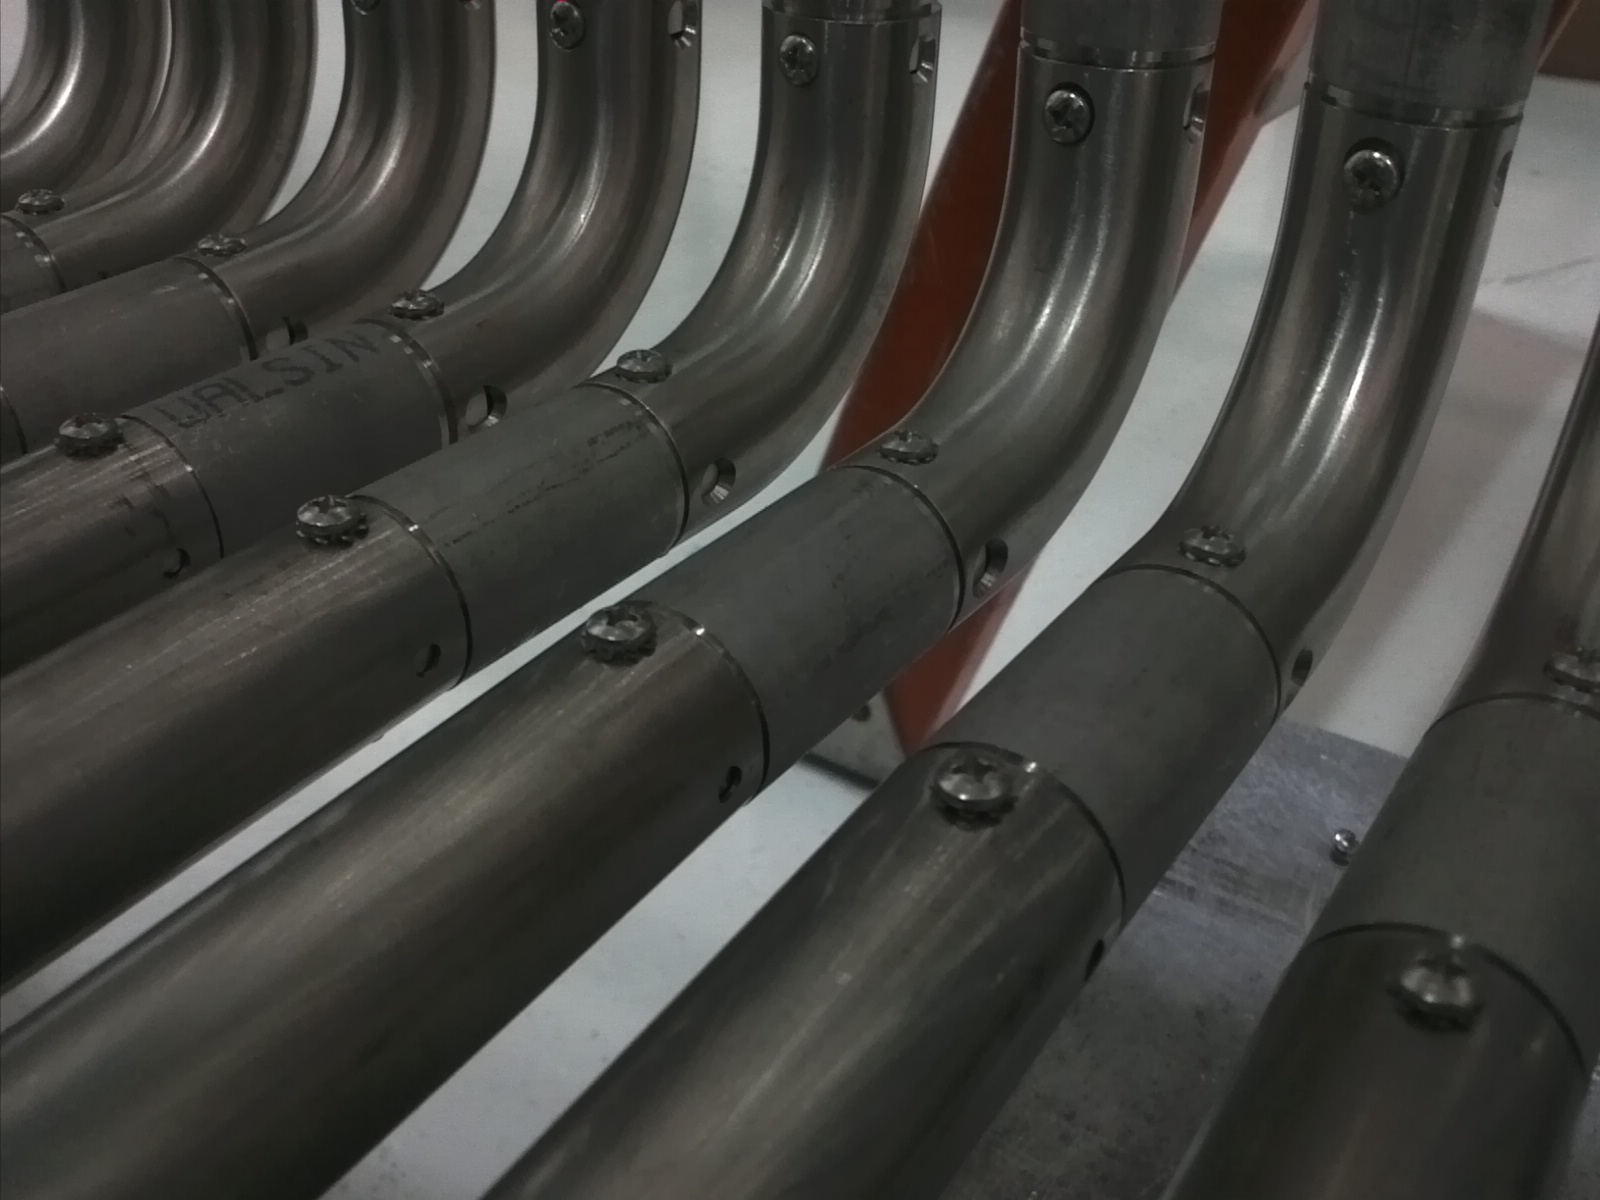
\includegraphics[width=0.9\linewidth]{figures/tpc-fieldcage-coupling.jpg}
\caption{Field cage loop corner, showing elbow and couplings.}
\label{fig:tpc-fieldcage-elbows}
\end{figure}

In order to avoid electrical breakdown between the inner cryostat surface and field cage parts at high potential on or near the cathode, the electric field strength is minimized at the corners and edges of the field cage. Loops 0, 1, and 2 are each designed differently than the other field cage loops.  Loop 0 is a special case in that it is made from larger diameter piping of 5.08 cm OD, and frames the cathode and also acts as its mechanical support.  It operates at the same electrical potential as the cathode plane sheets attached to it.  Loop 0 has a slightly smaller area than the other field cage loops, as shown in figure~\ref{fig:tpc-smooshed-elbow}.  Loop 1 is the first of the 64 loops in the field cage with 2.54 cm.  It surrounds the cathode plane and operates at cathode potential.  The elbow of loop 1 has a specially designed geometry in order to minimize the electric field potential.  The elbow of loop 2 has a softer radius of curvature than the standard elbows, also for the purpose of minimizing the electric field potential. For all three of these loops (loop 0, 1, and 2), connections at corners and joints are made by welding instead of screws to avoid sharp edges that would result in higher electric fields and greater chance of electrical breakdown.

\begin{figure}
\centering	
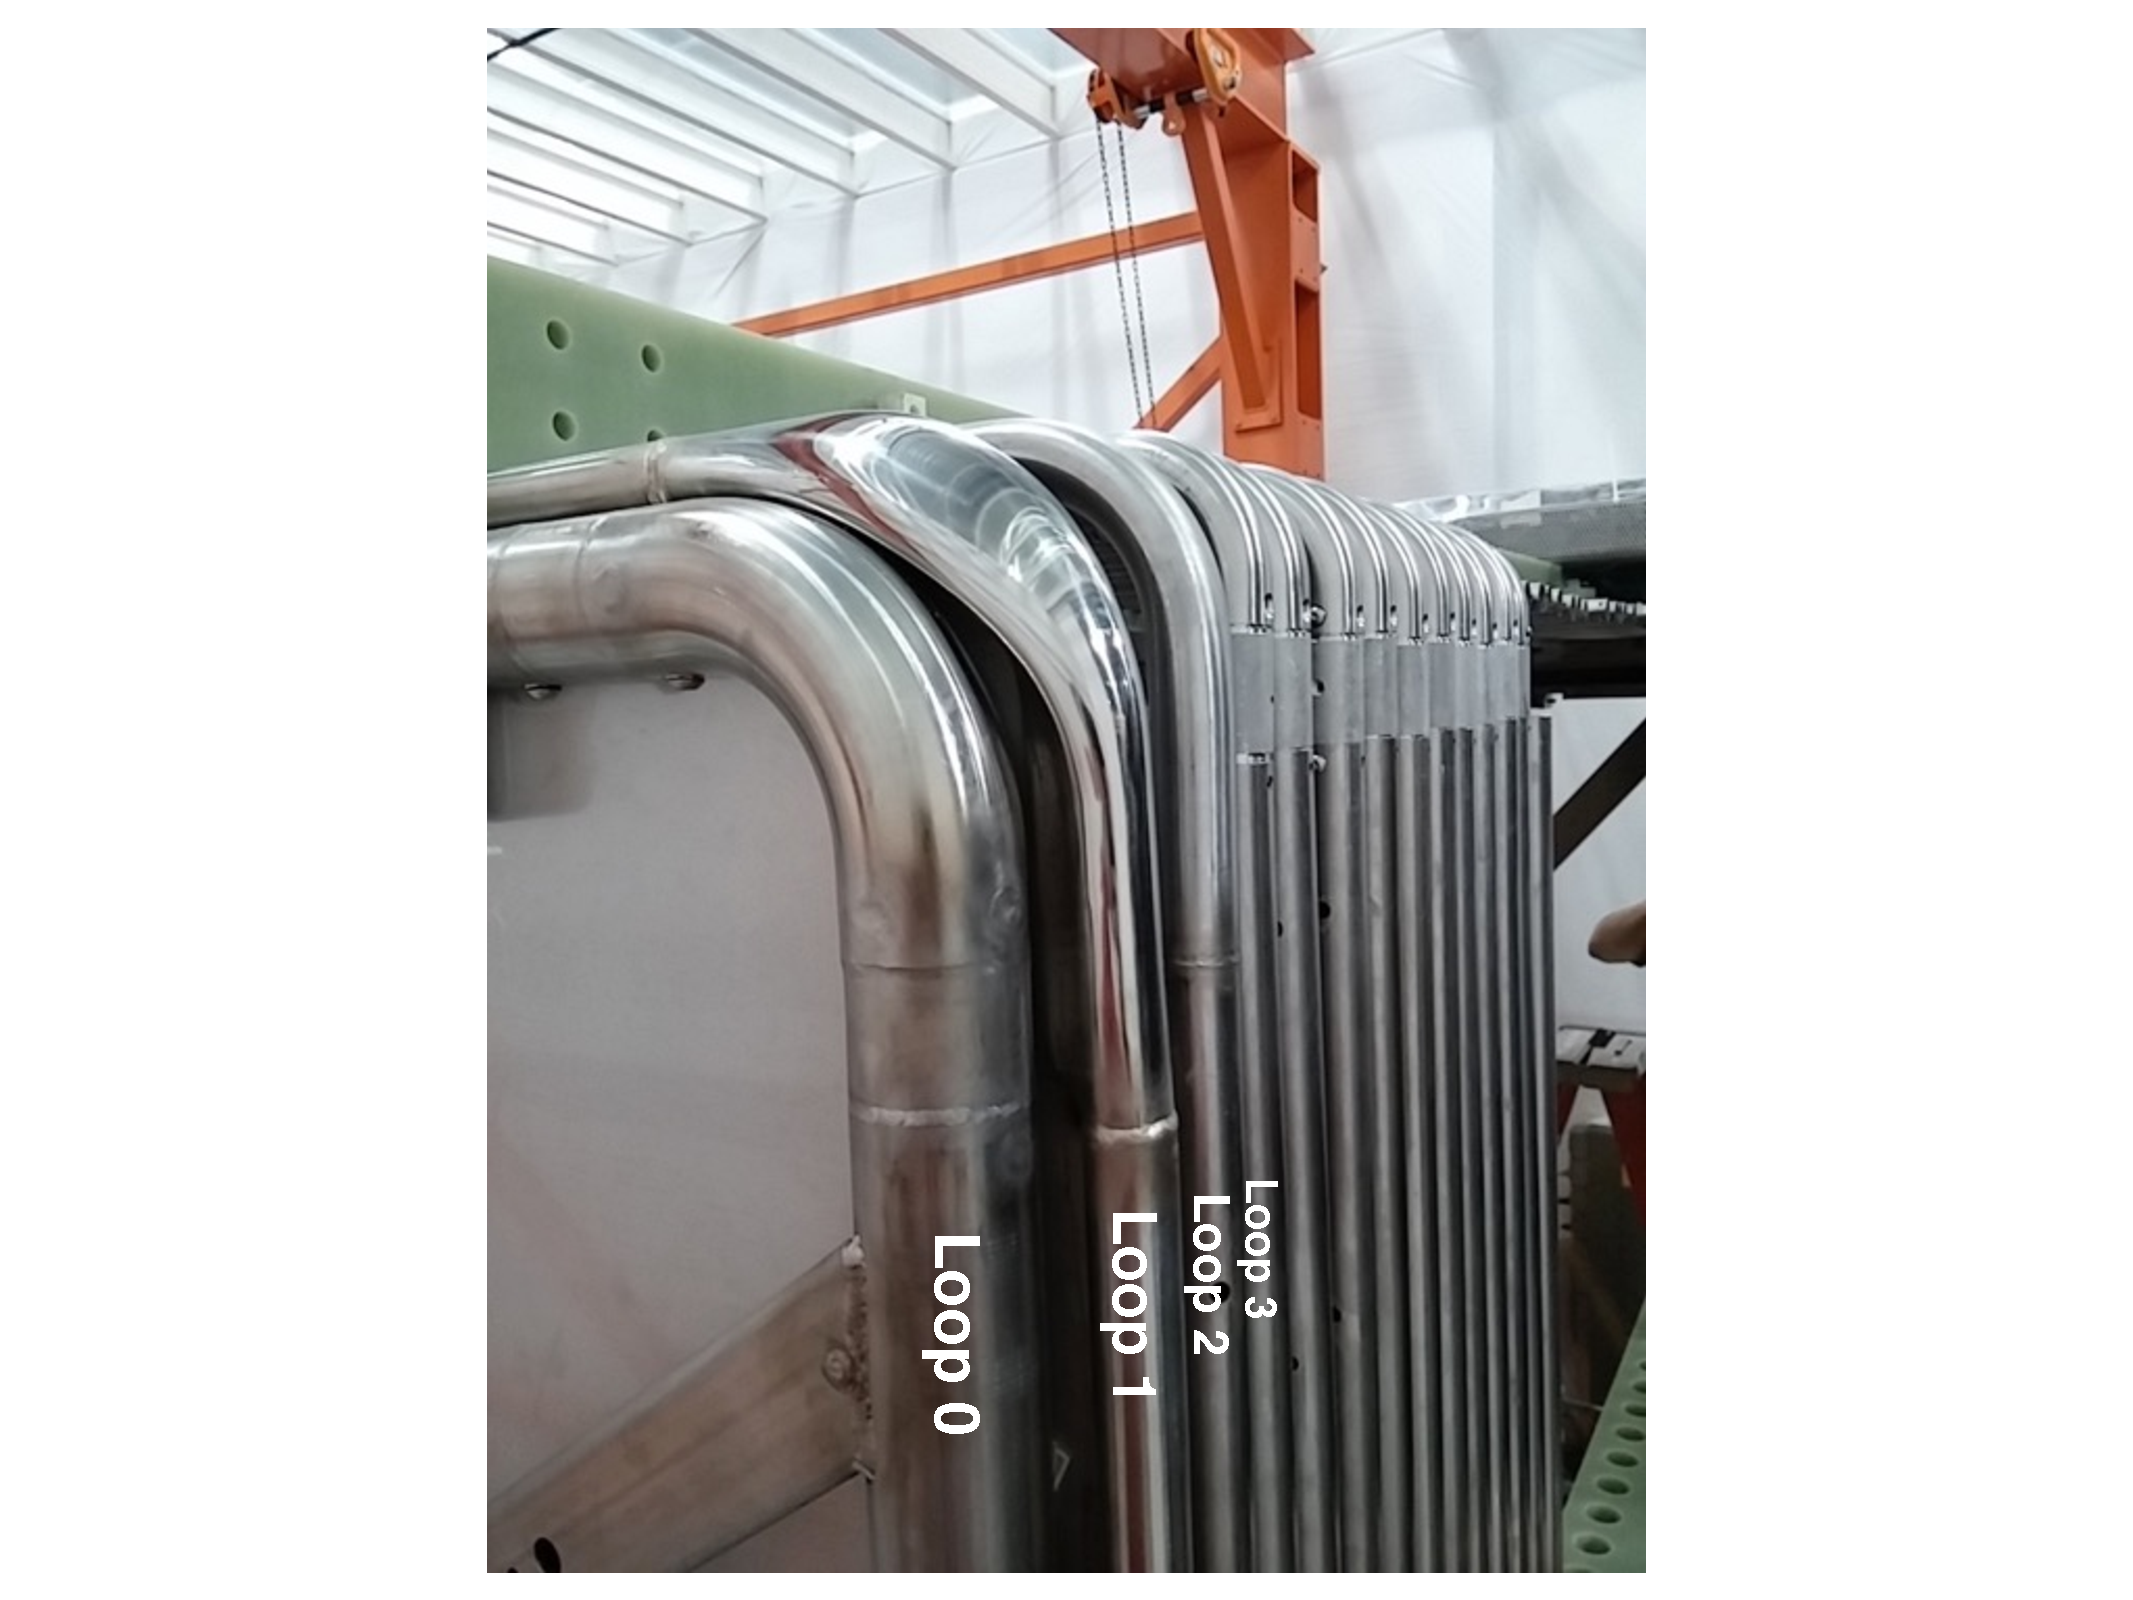
\includegraphics[width=0.7\linewidth]{figures/tpc-fieldcage-loops}
\caption{Photograph of the field cage during construction, with loops 0 (cathode) through 3 labeled.  Field cage loops closest to (and including) the cathode are modified to reduce sharp edges that would result in higher electric fields.}
\label{fig:tpc-smooshed-elbow}
\end{figure}

Another precaution to minimize the electrical field between the loops and the cryostat surface is the positioning of the coupling screws: for the first 20 loops, the screws are positioned on the sides facing the screws of the neighboring loops instead of facing inward to the \lartpc active volume and outward toward the grounded cryostat surface. Hex-head button-screws and lock washers are also used here in order to minimize sharp metal edges.

Figure \ref{fig:efield} shows the simulated electric field values inside the MicroBooNE \lartpc, and some of the surrounding volume inside the cryostat, when the cathode is set to an operating voltage of -128 kV.  

\begin{figure}
\centering	
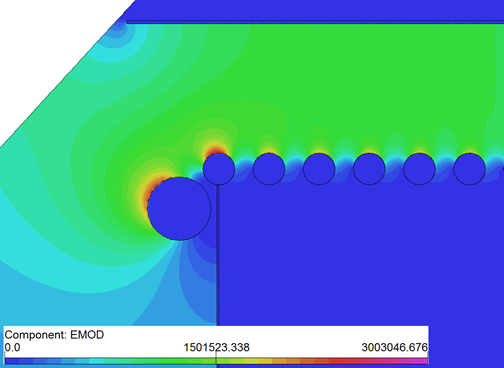
\includegraphics[width=0.7\linewidth]{figures/efield.png}
\caption{Cross-section view showing electric field simulation inside the field cage when the cathode is set to a voltage of -128 kV.  Loop 0 is represented by the larger diameter circle on the left of the image.  The legend shows the absolute values of electric field modulus in units of V/m.}
\label{fig:efield}
\end{figure}



\subsubsection{Resistor Divider Chain}
%{\it{Anne, Jen}}

A resistor divider chain installed across the field cage loops steps the voltage down in magnitude from the cathode plane to the anode wire plane in equal steps.  For a nominal value of -128~kV on the cathode, this results in a potential difference of 2~kV between each pair of loops. The value of the equivalent resistance between loops within the divider chain was chosen to be low enough such that the current flow through the divider circuit is much greater than the signal current flowing through the \lartpc. The signal current in our case is dominated by the free ionization produced by the cosmic ray flux, and is estimated to be <50~nA.  An equivalent resistance of 250~M$\Omega$ between each pair of field cage loops, corresponding to a current flow of 8~$\mu$A, was chosen.  

The voltage divider chain is mounted on the inside of the field cage at the upstream end of the detector. The couplings at the top corner of each field cage loop have additional holes facing the inside of the field cage, where the resistors are mounted. On the first 16 field cage loops, pairs of Metallux HVR 969.23 499~M$\Omega$ resistors (rated to 23~W, 48~kV in air) are mounted electrically in parallel to establish the beginning of the voltage divider chain. On the remaining loops, four thick-film Ohmite Slim-Mox 104E metal-oxide epoxy-coated resistors with a lower power and voltage rating (1.5~W, 10~kV in air) are mounted in parallel, per loop.  Extensive testing was done on these two types of resistors \cite{Bagby:2014wva}. 

%For redundancy, the desired 250~M$\Omega$ total resistance between each pair of field cage loops is composed of four individual 1~G$\Omega$ Slim-Mox 104E resistors placed electrically in parallel and attached to a printed circuit board. 

For the loops with the Slim-Mox resistors, printed circuit boards span across eight field cage gaps and therefore have eight 250~M$\Omega$ resistances in series, shown in figure~\ref{fig:tpc-voltage-divider-slimmox}. The electrical connection between the boards and each field cage loop is made by metal contact pads on the back side of the boards, held in electrical contact with the field cage tube by a hex-head button-screw and lock washer.

\begin{figure}
\centering	
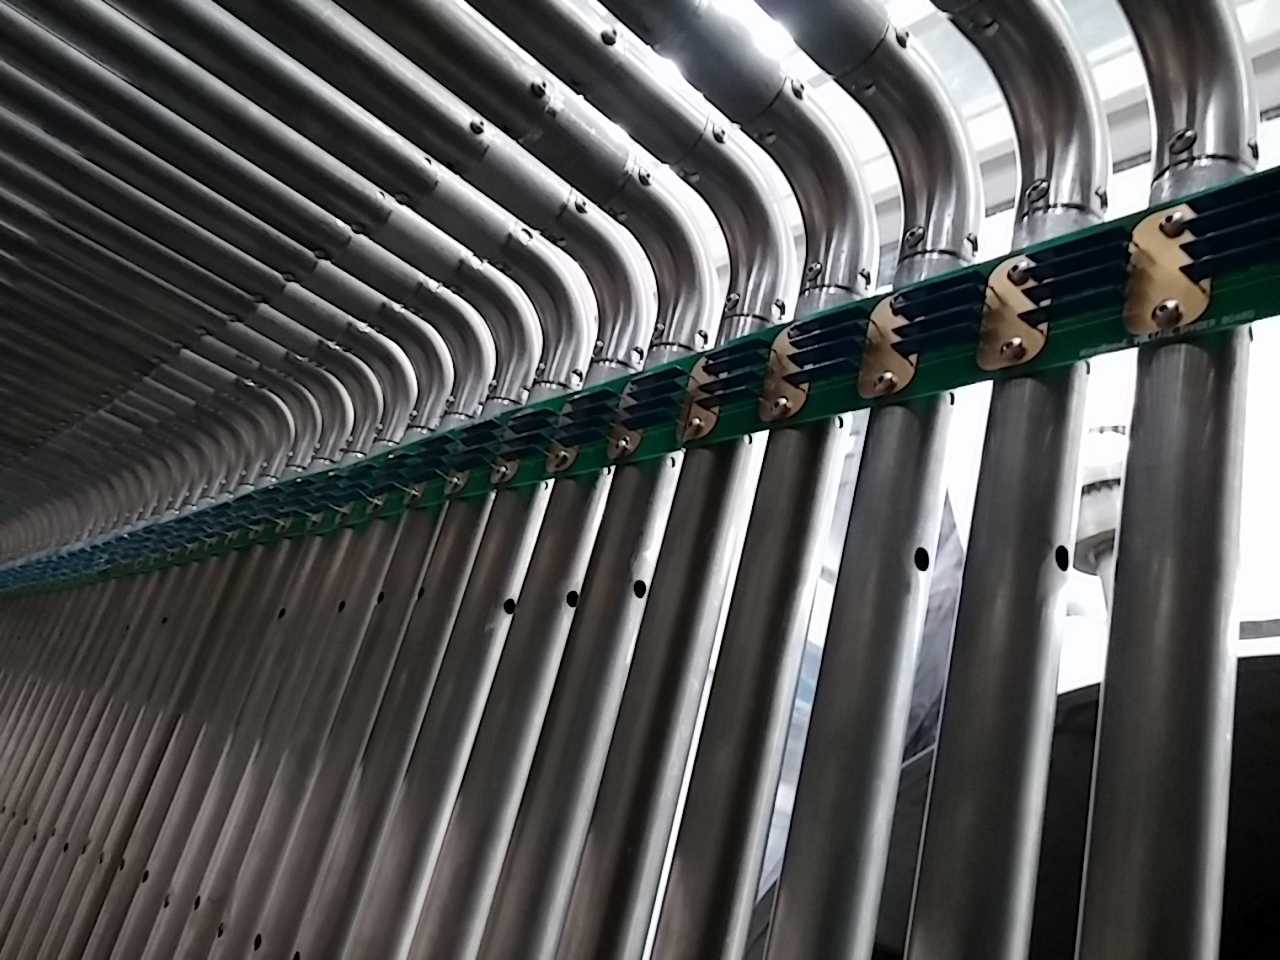
\includegraphics[width=0.8\linewidth]{figures/tpc-voltage-divider-slimmox.jpg}
\caption{The Ohmite Slim-Mox 104E resistors arranged in parallel sets of four on printed circuit boards that span eight field cage tubes.}
\label{fig:tpc-voltage-divider-slimmox}
\end{figure}

While the designed operating voltage difference across each resistor in the detector is 2~kV with a power flow of 4~mW, there is a slight possibility that the voltage drop and power could temporarily exceed the rating of the resistors in the case of discharge between the cathode plane or field cage loops and the cryostat wall, through the bulk liquid argon. Recent studies~\cite{Acciarri:2014ica} have shown that the value of the minimum breakdown electrical field decreases with the increasing argon purity; for purities as high as that required in the MicroBooNE detector, breakdown has been observed at electric fields as low as 40~kV/cm.

The field cage behaves like a capacitance network at high frequencies. Based on measurements and simulations, the total energy stored inside the field cage when fully charged is estimated to be approximately 24~J. In the case of a discharge between the cryostat and the cathode or one of the field cage loops close to the cathode, simulations show that voltages of up to 80~kV peak, with a discharge time constant of a few seconds, can develop across the resistors. The observed peak voltages in such discharge scenarios decrease the further the breakdown occurs from the cathode, such that discharges occurring between the cryostat and field cage loops 32 through 63 do not exceed the 10~kV rating of the resistors.

Two strategies have been implemented to protect the resistors nearest to the cathode from damage due to discharge.   The first is the use of the Mettalux resistors on the first 16 loops given their higher voltage rating of 48~kV as compared to the Slim-Mox resistors on the remaining loops.      


%In order to protect the resistors near the cathode from damage which could potentially render the field cage inoperable, two strategies have been implemented.   First, on the first 16 field cage loops near the cathode the Ohmite Slim-Mox 104E resistors are replaced by 499~M$\Omega$ Metallux HVR 969.23 resistors that have a higher voltage rating of 48~kV. An extensive study of resistor breakdown in liquid argon of several resistor brands and models \cite{Bagby:2014wva} has revealed that the breakdown voltage observed in liquid argon exceeds the rating in air substantially for all resistors. No breakdown has been observed up to 32~kV for the Ohmite Slim-Mox 104E resistor. For the Metallux HVR 969.23 resistors, no breakdown has been observed up to the limit of the test apparatus of 130~kV.  

Since the Metallux HVR 969.23 resistors are significantly larger physically than the loop-to-loop distance, they are mounted diagonally between each pair of field cage loops. They are held by copper brackets, which are attached to studs welded onto the field cage tubes, shown in figure~\ref{fig:tpc-voltage-divider-metallux}.

\begin{figure}
\centering	
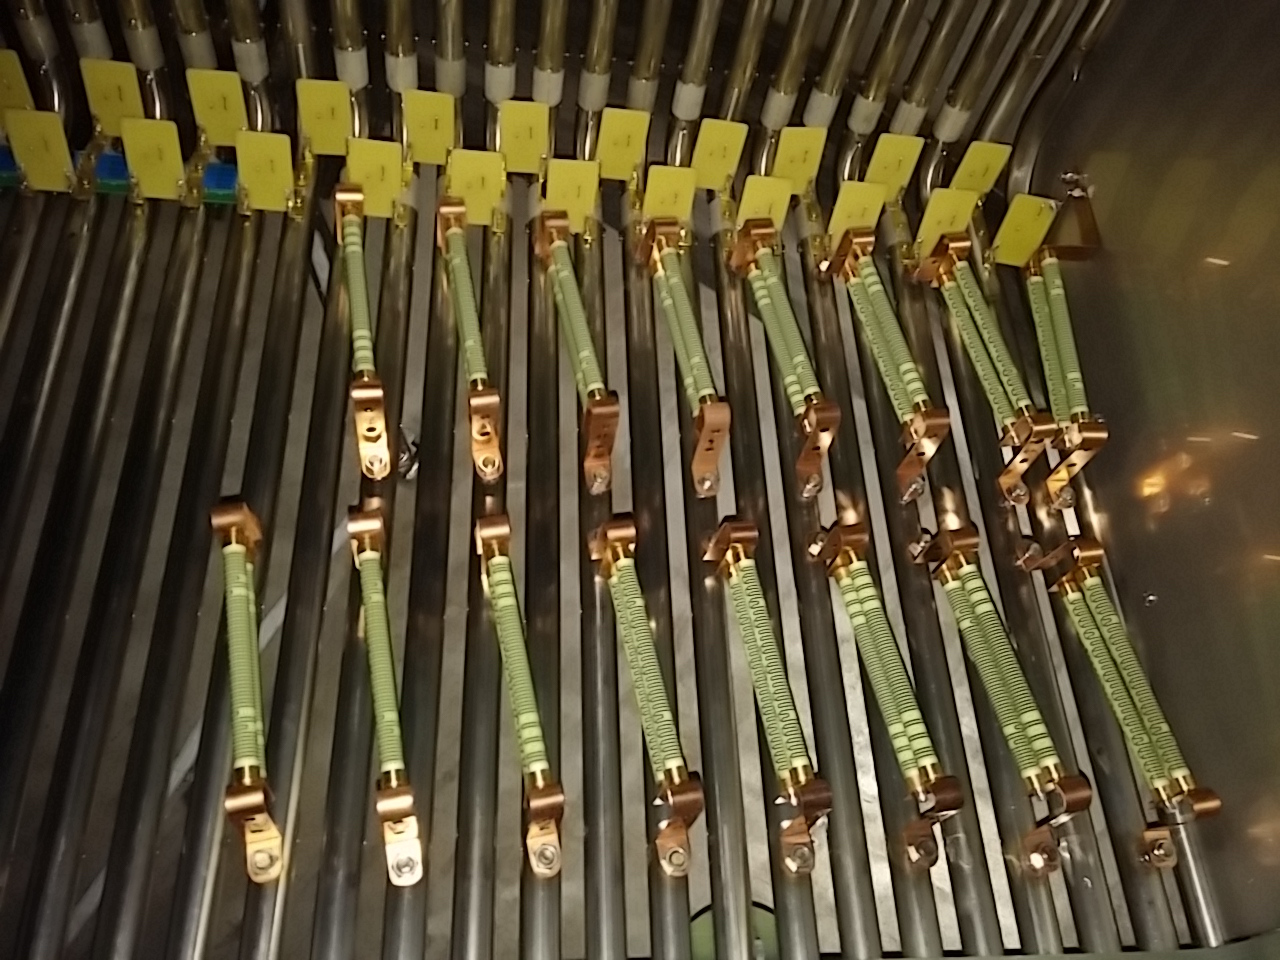
\includegraphics[width=0.8\linewidth]{figures/tpc-voltage-divider-metallux.jpg}
\caption{The Metallux HVR 969.23 resistors mounted on the 16 field cage loops closest to the cathode.}
\label{fig:tpc-voltage-divider-metallux}
\end{figure}


The second is installation of surge protection curciuts on field cage loops 1 through 32.  The chosen surge protection devices are designed to short the circuit in the case of a voltage spike, which protects any other electrical components installed in parallel.  Below their clamping voltage, they exhibit a very high resistance and do not influence the circuit. The behavior of Gas Discharge Tubes (GDTs) and varistors in liquid argon has been studied extensively for application in the MicroBooNE field cage \cite{Asaadi:2014iva}. The surge protection device chosen is a Panasonic ERZ-V14D182 varistor with a clamping voltage of 1700 V. In order to obtain a very high resistance in normal operation and a clamping voltage above the 2~kV in normal operation mode, three of these devices are mounted in series across a block of four Slim-Mox 104E or two Metallux 969.23 resistors. These additional varistor boards make electrical contact with the field cage via brass mounting brackets that are fastened to the field cage with button-head screws, as shown in figure~\ref{fig:tpc-voltage-divider-varistors}.

\begin{figure}
\centering	
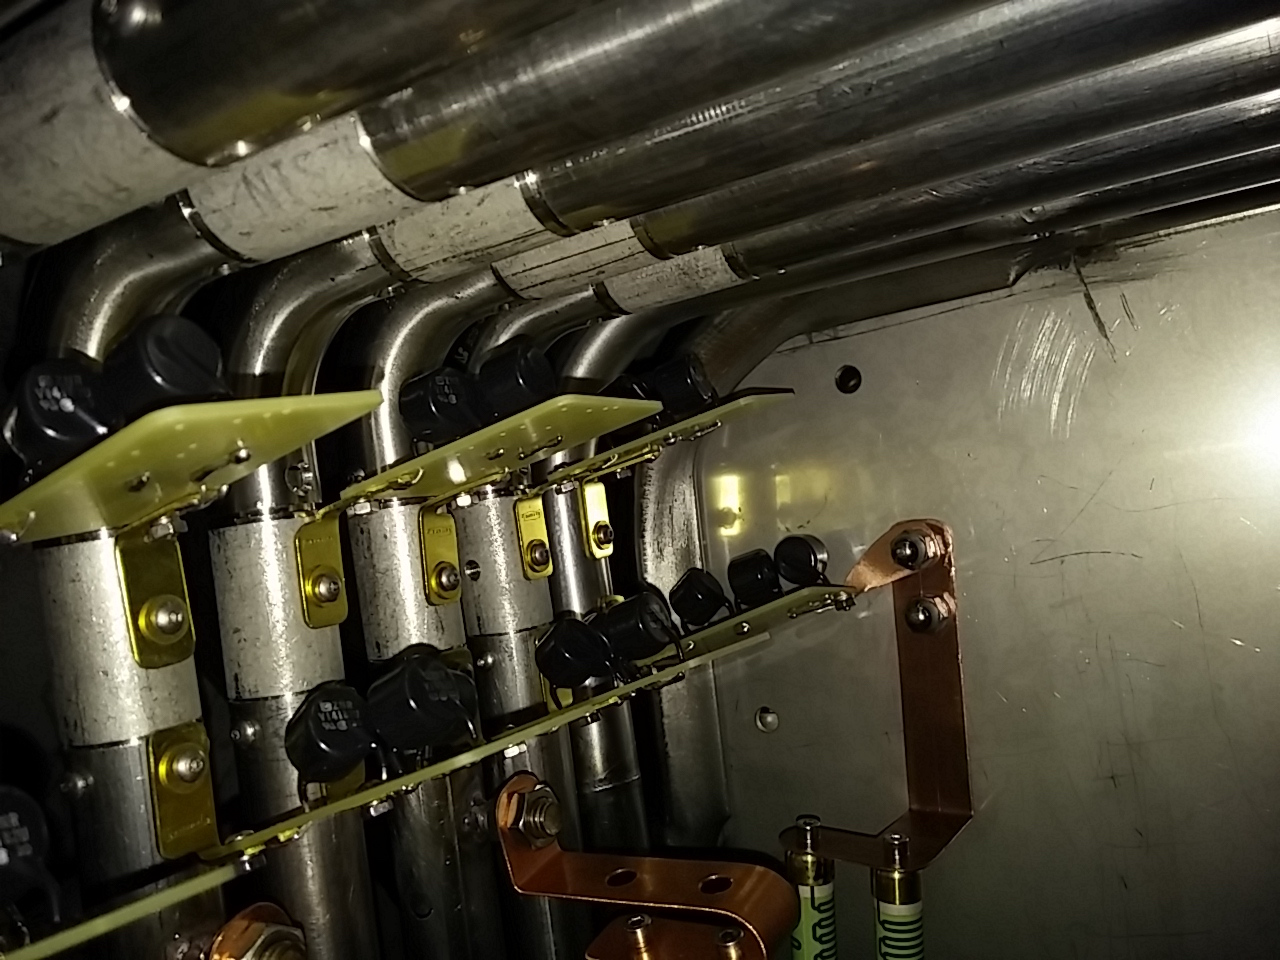
\includegraphics[width=0.8\linewidth]{figures/tpc-voltage-divider-varistors.jpg}
\caption{Surge-protecting varistors are installed in parallel with the voltage divider resistors for the first 32 field cage loops. Here, they are shown mounted on small boards in sets of 3, and attached to the field cage by means of 6-32 hex button head screws.}
\label{fig:tpc-voltage-divider-varistors}
\end{figure}


%Comment from Anne:{\it{ Do we want to talk in more detail about the simulations for discharge? Is this enough "material science detail" about the resistors and varistors?  We put a lot of additional thoughts in the mounting: Positioning near resistors, heat development, bubbles, venting, cooldown contraction … do we want to mention this?}}



\subsection{Anode Planes}
%{\it{Bo, Jen}}

The anode frame holds the induction and collection plane sense wires at tension and provides overall structural support for the beam-right side of the LArTPC.  Individual sense wires for all anode planes are held in place by wire carrier boards, which are printed circuit board assemblies that locate the wires as well as provide the electrical connection to the electronic readout system of the experiment.

\subsubsection{Mechanical structure}

The anode frame is comprised of a stainless steel C-channel hosting adjustable tensioning bars to which the wire carrier boards are attached. The C-channel and tensioning bar assembly is depicted for one corner of the anode frame in figure~\ref{fig:anode-frame-3dmodel}.  Wire carrier boards attach to precision alignment pins distributed along the length of the tensioning bars. 

\begin{figure}
\centering	
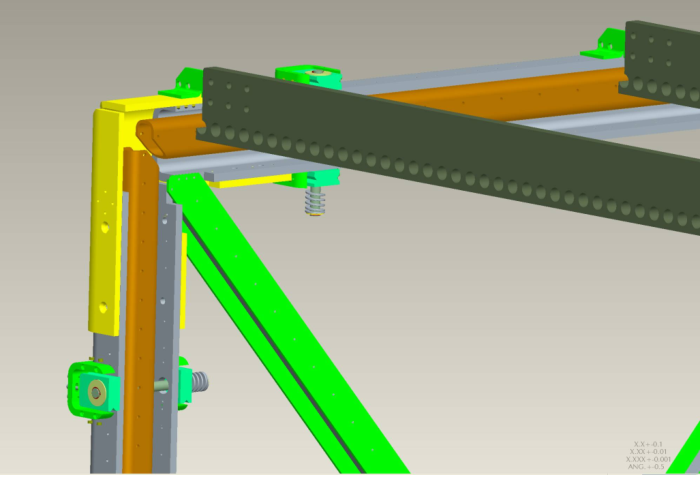
\includegraphics[width=0.8\linewidth]{figures/anode-frame-3dmodel.pdf}
\caption{Rendering of the anode frame assembly.  The C-channel is depicted in gray, and the adjustable tensioning bar assembly is shown in orange.}
\label{fig:anode-frame-3dmodel}
\end{figure}

\subsubsection{Wire winding and quality assurance}
%{\it{Roxanne (and Corey?)}}

The three anode planes are constructed from wire carrier boards that had individually-prepared wires attached to them in groups of 16 (for the U- and V- angled planes) or 32 (for the vertical Y-plane).  Consistent quality in wire preparation was achieved by a semi-automated winding machine, which terminated the ends of each wire via wrapping around 3~mm diameter brass ferrules as shown in figure~\ref{fig:ferrules}.   The wire termination method via wrapping around a brass ferrule is like that done on the ICARUS T600 detector.  
\begin{figure}
\centering
%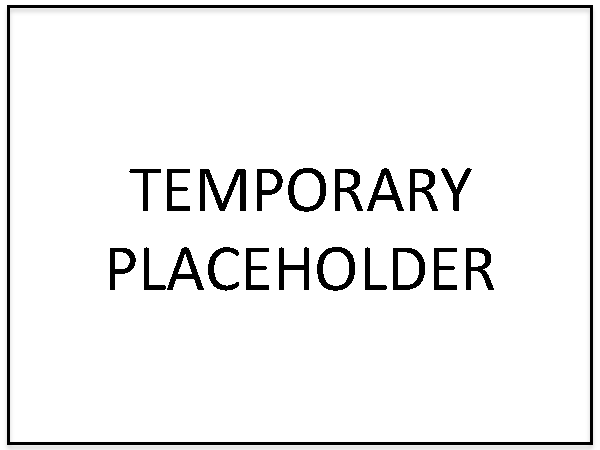
\includegraphics[width=2in]{figures/temp.pdf}
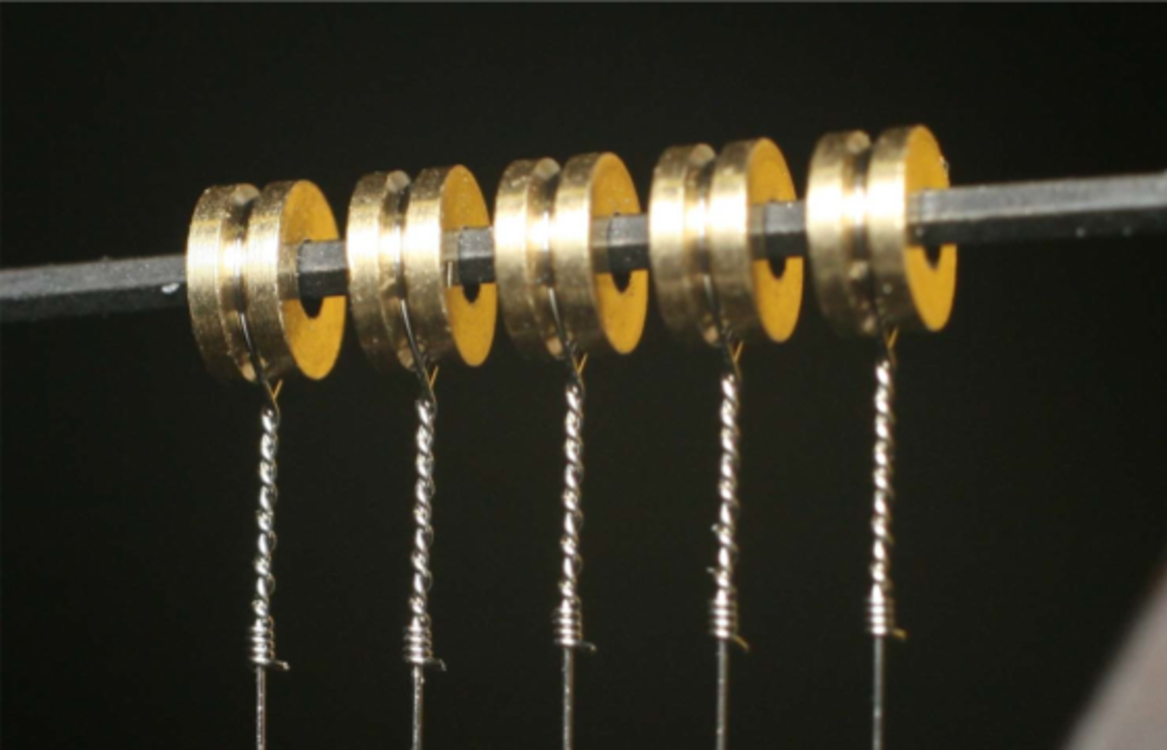
\includegraphics[width=0.5\textwidth]{figures/wire-twist.pdf}
\caption{Photograph of the wire termination on the brass ferrules.  Each ferrule is 3~mm in diameter, and 1.5~mm thick.}
\label{fig:ferrules}
\end{figure}

Each wire was tested for strength on a tensioning stand where a load of 2.5~kg (more than 3 times the nominal load of 0.7 kg) was applied for 10 minutes, ensuring that the wire preparation did not leave any weaknesses that could result in a breakage.  Upon successful completion of the quality assurance testing, each wire was placed onto a wire carrier board, shown in figure~\ref{fig:carrier-boards}.


\begin{figure}
\centering
%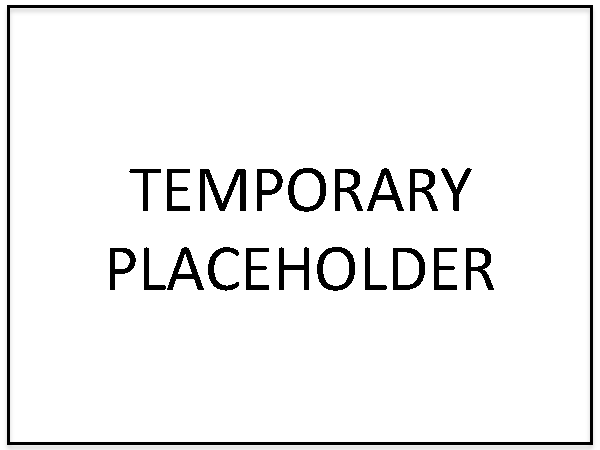
\includegraphics[width=2in]{figures/temp.pdf}
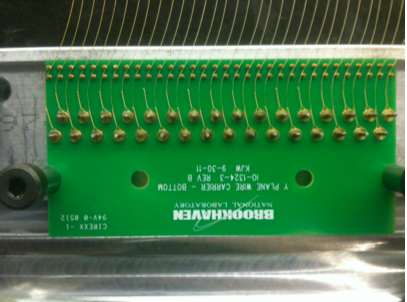
\includegraphics[angle =0,width=0.7\textwidth]{figures/wire-carrierboard.png}
\caption{Photograph of a collection plane wire carrier board that has been filled with wires, but has not yet had the cover plate installed.}
\label{fig:carrier-boards}
\end{figure}


When installed on the wire carrier boards, the wires make contact with gold pins which are connected to a trace that routes to the cold electronics.  Once the wire-carrier board was filled with wires, a cover plate was installed and press-fit rivets were installed to hold the assembly together. The assembled wire carrier board was then placed onto a tension stand, to reapply a 2.5 kg tension/wire to the whole board for 10 minutes. This is to ensure that the wires were not weakened during the board assembly process. The tension stand is depicted in figure \ref{fig:stress-stand}.   A comprehensive description of the MicroBooNE wire preparation and associated quality assurance studies can be found in \cite{Acciarri:2016ugk}.

\begin{figure}
\centering
%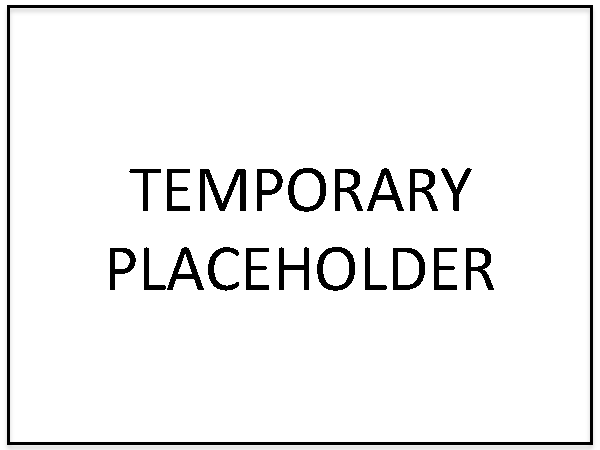
\includegraphics[width=2in]{figures/temp.pdf}
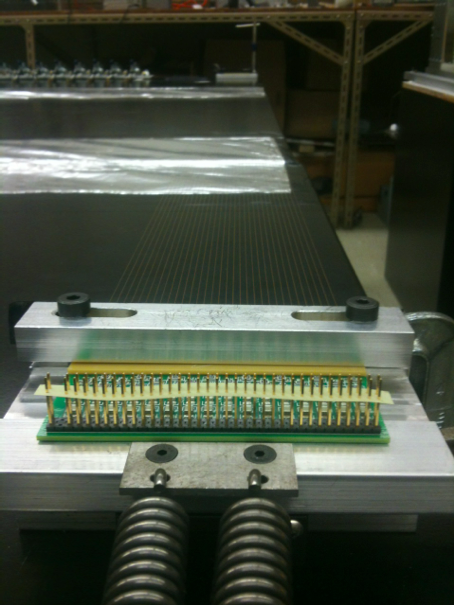
\includegraphics[angle=0,width=0.5\textwidth]{figures/wire-boardtension.png}
\caption{Photograph of a collection plane wire carrier board on the tension stand.}
\label{fig:stress-stand}
\end{figure}



%\input{tpc-prep}
\subsection{Parts Preparation}
%{\it{(More details in internal uB note: DocDB 2259, also 1820, 1922, 1923)}}

The majority of the parts that make up the \lartpc are either stainless steel or G-10. These two material types, as well as any others used in the LArTPC, were tested in the Fermilab Materials Test Stand (MTS)~\cite{Rebel:2011-MTS}, whose purpose was to investigate the suitability of materials for use in LArTPCs.  The MTS confirmed that none of the materials used in the \lartpc assembly would contaminate the liquid argon.  Before assembly, all \lartpc parts were cleaned according to the procedures described in the following sections.

\subsubsection{Cleaning stainless steel}

The delivered stainless steel parts were often greasy due to machining, and those with holes or interior cavities generally had a significant amount of trapped metal shavings due to the machining processes. Many of the pieces also had markings from permanent ink pens, dirt smears, rust spots, and/or dried oil from machining. These pieces were scrubbed with ScotchBrite 7447 general-purpose hand pads before cleaning.

Parts that were small enough to fit in an ultrasonic bath were prepared according to the following prescription. A pre-rinse with tap water was performed to remove particulate matter, followed by deburring of sharp edges. The first ultrasonic wash was 15 minutes in heated distilled water with a 3\% solution of Citranox acid detergent~\cite{citranox}. After a first rinse in distilled water, a second ultrasonic wash was performed, again for 15 minutes, but using heated distilled water with a weak solution of Simple Green detergent~\cite{simplegreen}. A second rinse in distilled water was performed, followed by a final rinse in a fresh bath of distilled water. The parts were then wiped dry with lint-free cloths, air dried completely, and wrapped in plastic film for storage.

Stainless steel parts that were too large to fit in the ultrasonic bath were prepared by a simpler prescription out of necessity. A pre-rinse with tap water was followed by deburring to remove sharp edges. Both the first and second washes were done with tap water and a weak solution of Simple Green detergent, scrubbing with brushes and lint-free sponges. Two tap water rinses were done, and the parts were then wiped dry with lint-free cloths. As a final additional step, each part was wiped with 200-proof ethyl alcohol, and then air dried completely. These parts were also wrapped in plastic film for storage.

\subsubsection{Cleaning G-10}

G-10 is known to absorb large quantities of water, which would outgas in the argon and could inhibit reaching the required argon purity in the detector. For this reason all G-10 parts were cleaned and then baked to remove moisture. The largest G-10 parts on the detector are beams that span the distance between the cathode and anode. These were washed in 1900-liter ultrasonic baths that are overseen by Fermilab Accelerator Division, typically used for cleaning large sections of accelerator beam pipes. An initial pre-wash was done with tap water to remove as much particulate matter as possible, since the machining process left a large amount of dust on the machined edges.  Pieces were then placed in the ultrasonic bath with heated deionized water and a 2\% solution of Elma Clean 65 (EC 65) neutral cleanser~\cite{elmaclean}. Two ultrasonic bath rinses were performed, and the pieces were then sealed in plastic bags with clean dry nitrogen gas. In order to remove the absorbed water, the large G-10 parts were then transported to the Fermilab Technical Division where they underwent an outgassing procedure to remove any remaining absorbed moisture.  They were baked in a large oven under vacuum until a plateau in the outgassing rate was reached, as reported by a monitor inside the oven. Upon completion of the outgassing procedure, the parts were resealed in plastic bags for storage.

\subsection{Assembly}
\label{sec:assembly}
%\paragraph{Mechanical structure}
%{\it{Overview of assembly steps (Jen)}}

The full mechanical structure of the \lartpc is shown in figure~\ref{fig:tpc-full}, with the left image depicting the cathode frame as semi-transparent to show the support structures on which the cathode sheets are attached. The anode frame is on the right of this image, with I-beams configured in a crossed pattern to maintain the shape and rigidity of the outer C-channel structure. Ribs of G-10 connect the anode and cathode, electrically isolating them from each other while also providing mounting holes to hold in place each of 64 field cage loops that define the active volume of the LArTPC.  The field cage loops are visible in the photograph on the right of figure~\ref{fig:tpc-full}.

\begin{figure}
\centering	
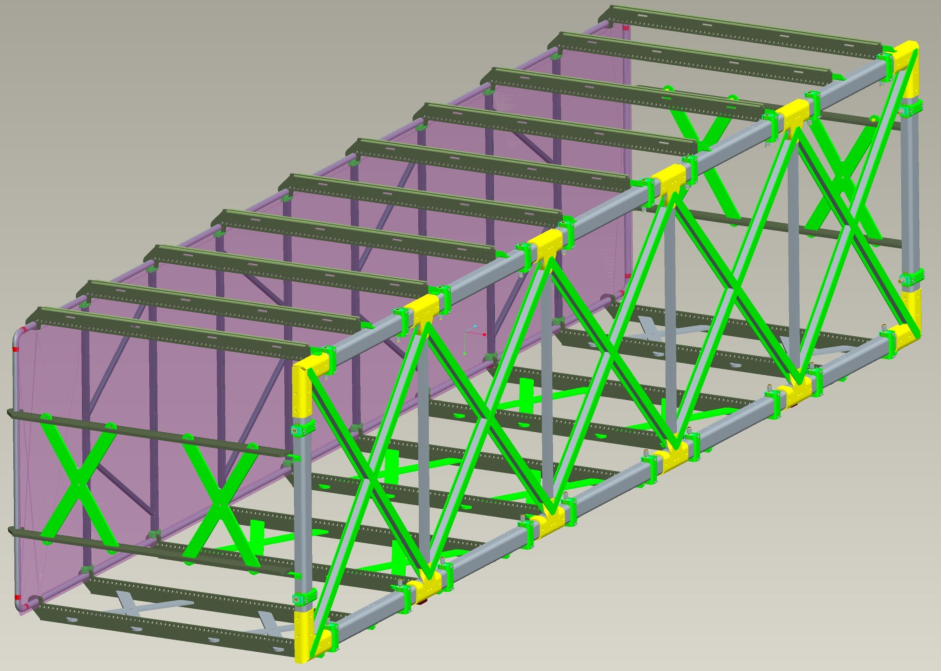
\includegraphics[width=0.48\linewidth]{figures/tpc-3drendering.pdf}
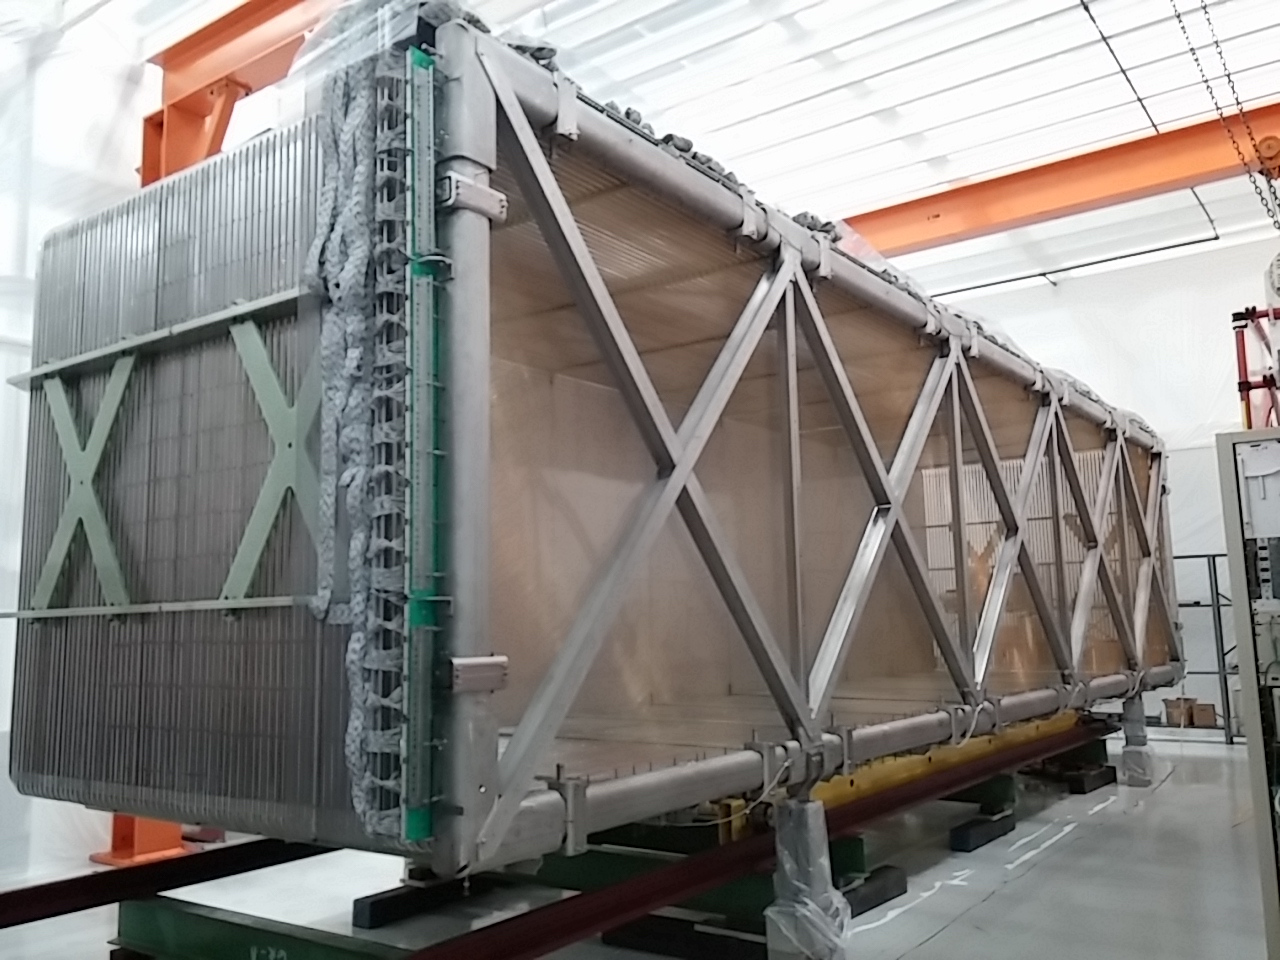
\includegraphics[width=0.48\linewidth]{figures/tpc-completed-upstream-right.jpg}
\caption{Top: Rendering of the full \lartpc frame assembly.  Bottom: Assembled \lartpc after wire and electronics installation.}
\label{fig:tpc-full}
\end{figure}

Assembly was done inside of a clean tent, shown on the top left in figure \ref{fig:tent}, on a flat surface made up of adjustable-height metal platforms that were installed on the assembly room floor.  These platforms were leveled to better than 0.5~mm before beginning assembly.  The anode frame was the first part of the detector to be assembled on this surface, shown on the top right of figure~\ref{fig:tent}. It was temporarily placed aside, and the cathode frame was assembled on the same set of platforms along with the G-10 ribs, which stood vertically with the help of temporary unistrut support pieces.  The combined cathode and G-10 frame was then lifted and rotated to the proper orientation, with G-10 ribs extending horizontally from the cathode to the anode, as shown on the bottom in figure~\ref{fig:tent}. Finally, the anode frame was brought back over and attached to the G-10 ribs, and the stainless steel tubes that make up the field cage loops were fed through the holes in the G-10 ribs to complete the mechanical structure of the LArTPC. 

\begin{figure}
\centering	
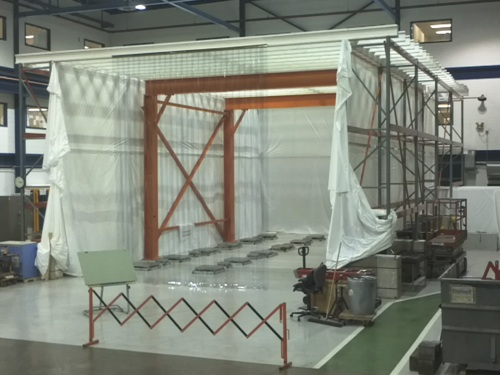
\includegraphics[width=0.48\linewidth]{figures/tent.jpg}
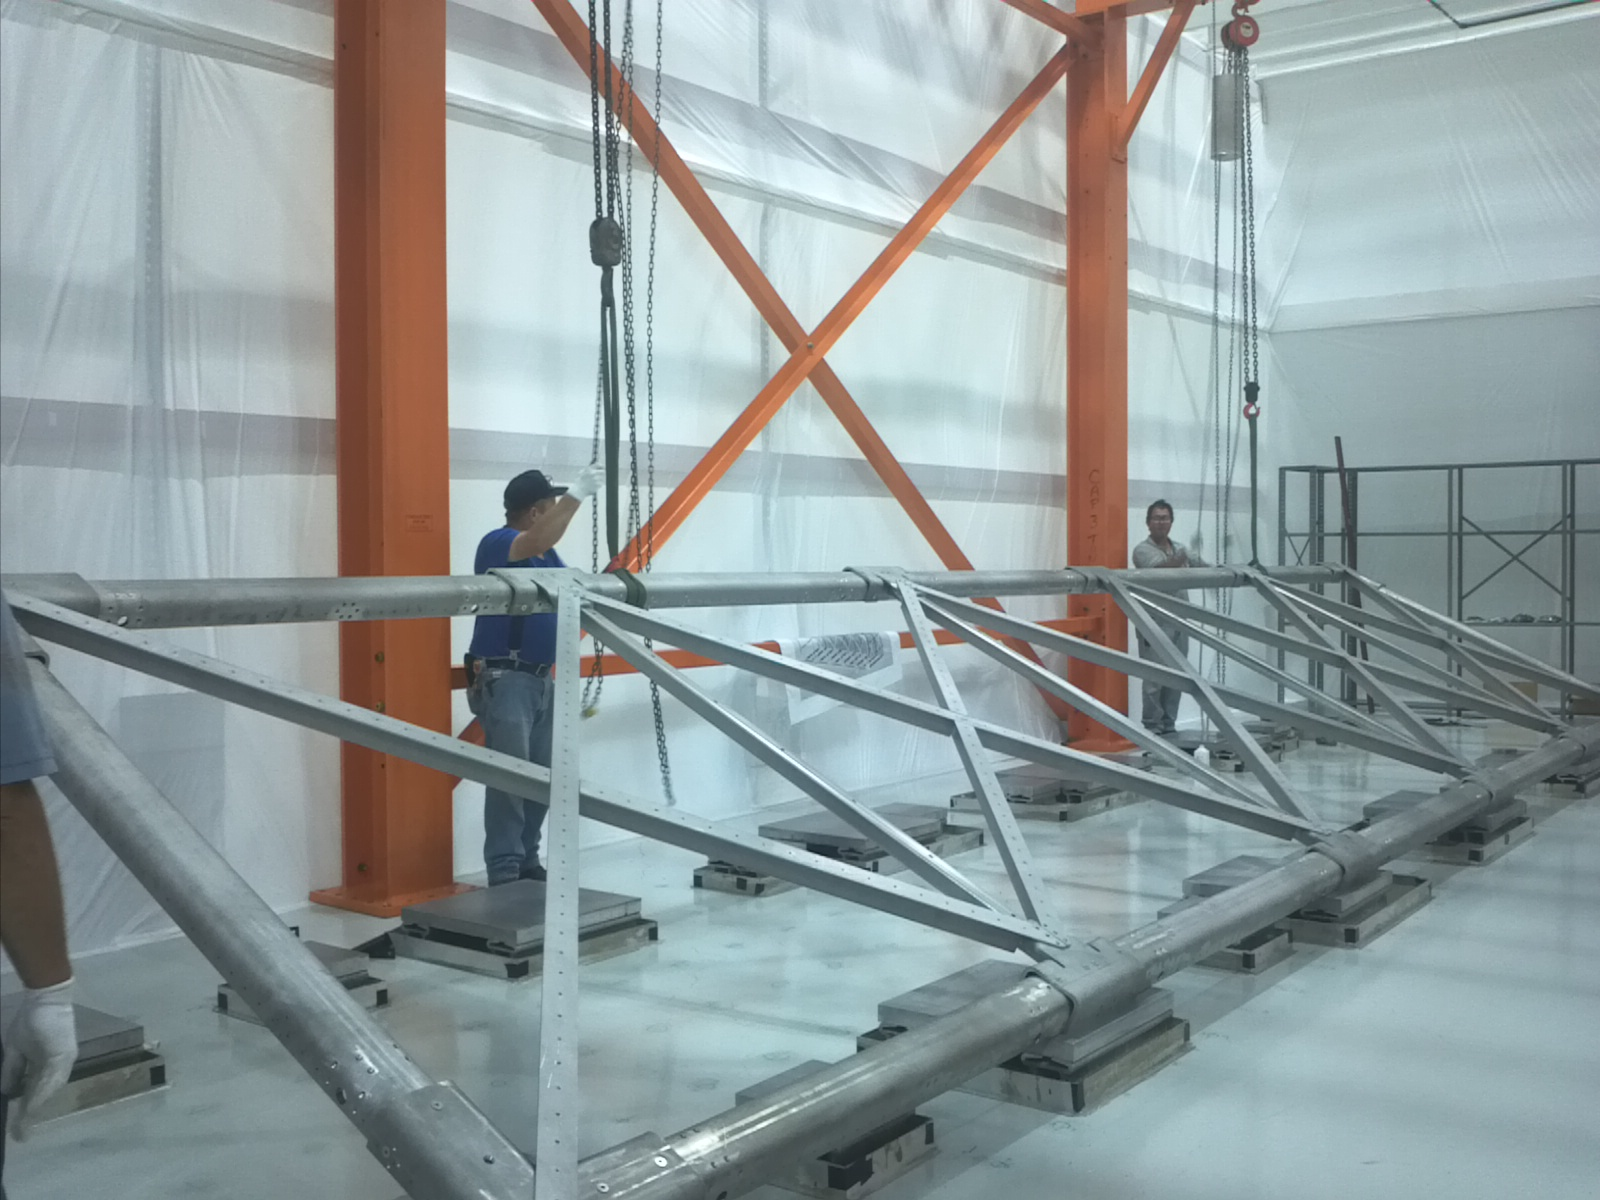
\includegraphics[width=0.48\linewidth]{figures/tpc-anode-frame.jpg}
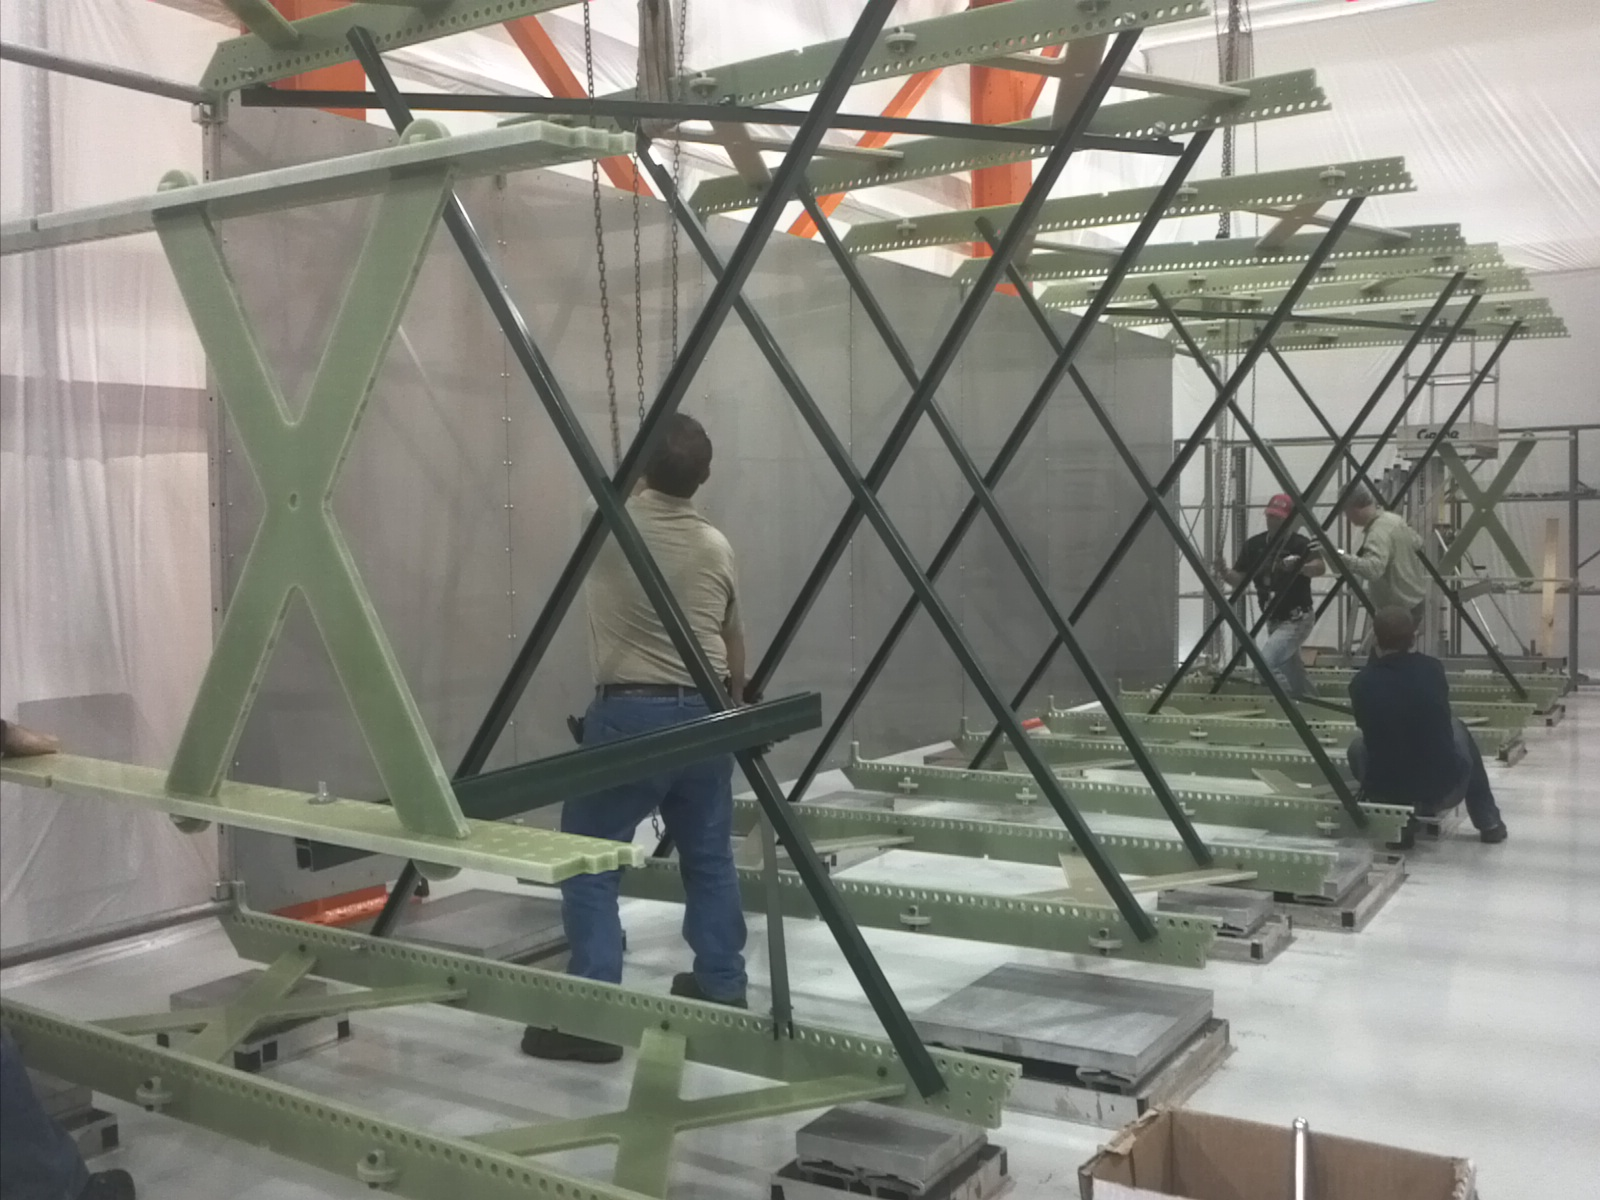
\includegraphics[width=0.48\linewidth]{figures/tpc-cathode-g10-frame.jpg}
\caption{Top Left: Clean tent where MicroBooNE \lartpc assembly was conducted. Top Right: Anode frame in the process of being moved from the metal assembly platforms. Bottom: Cathode frame and G-10 ribs on metal assembly platforms.}
\label{fig:tent}
\end{figure}


%\begin{figure}
%\centering	
%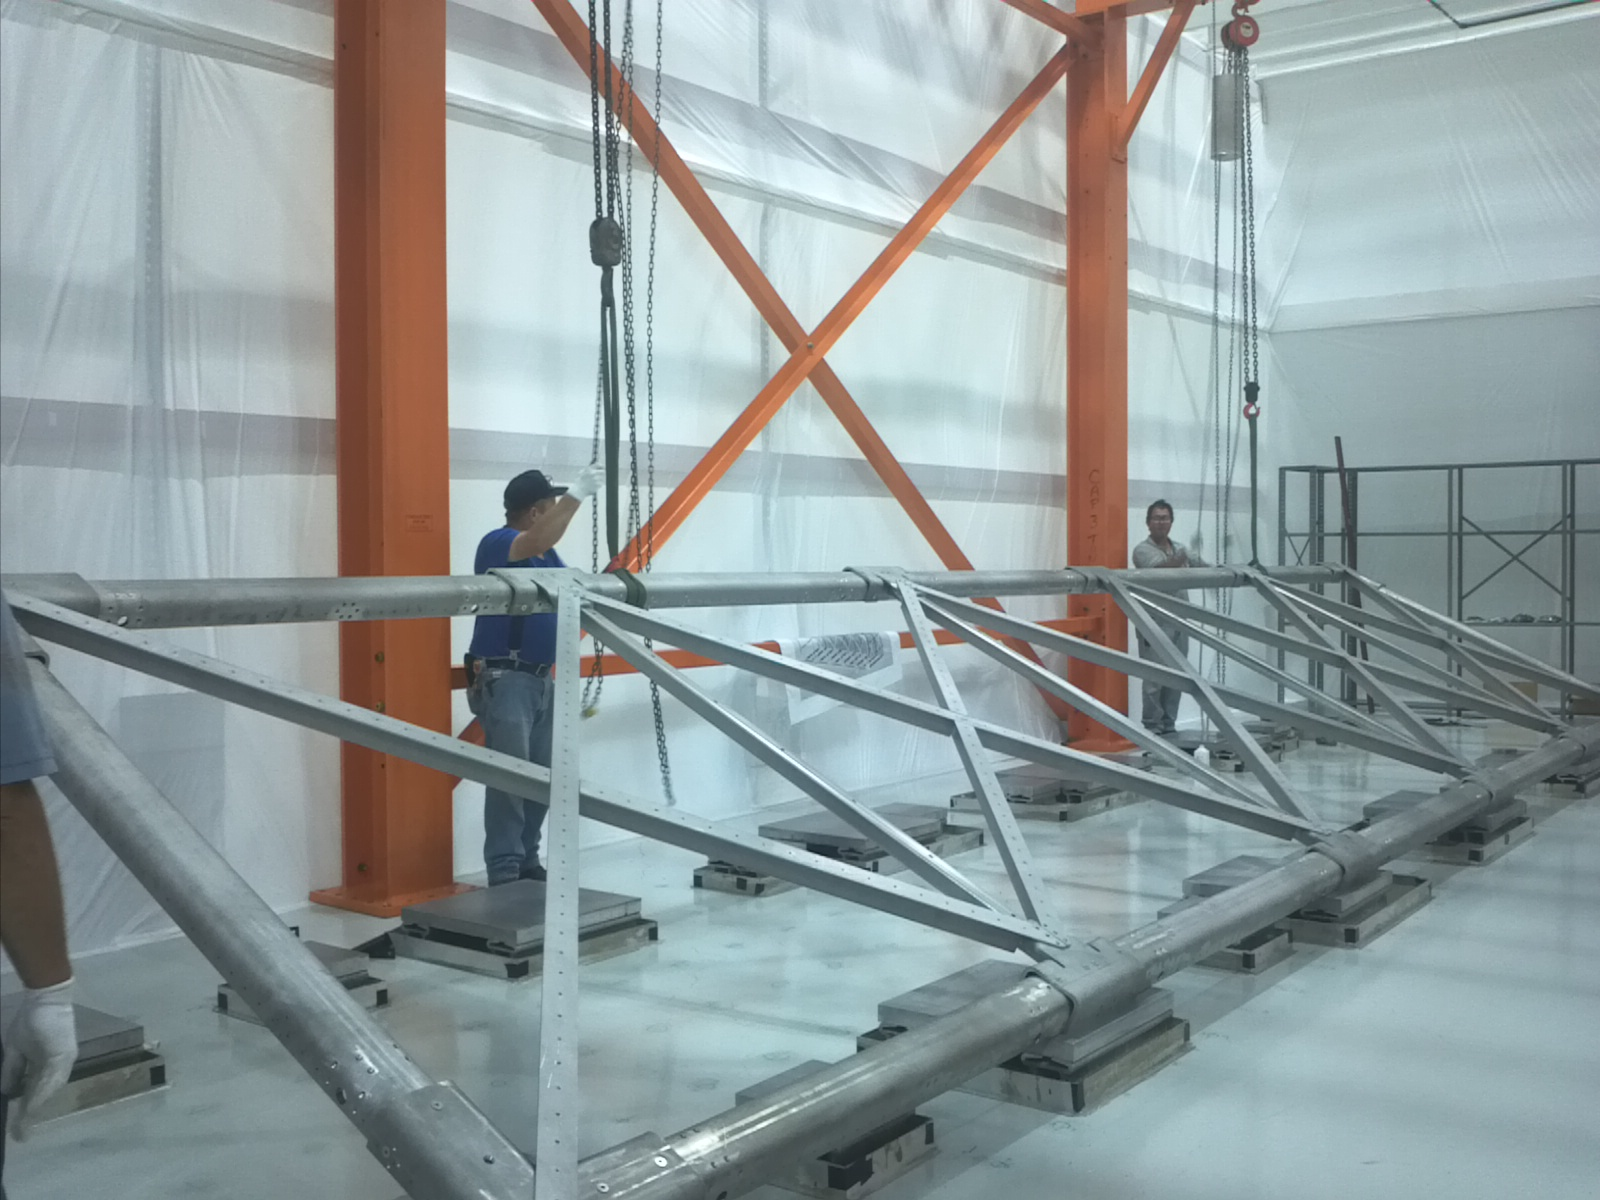
\includegraphics[width=0.7\linewidth]{figures/tpc-anode-frame.jpg}
%\caption{Anode frame in the process of being moved from the metal assembly platforms.}
%\label{fig:tpc-anode-frame}
%\end{figure}

%\begin{figure}
%\centering	
%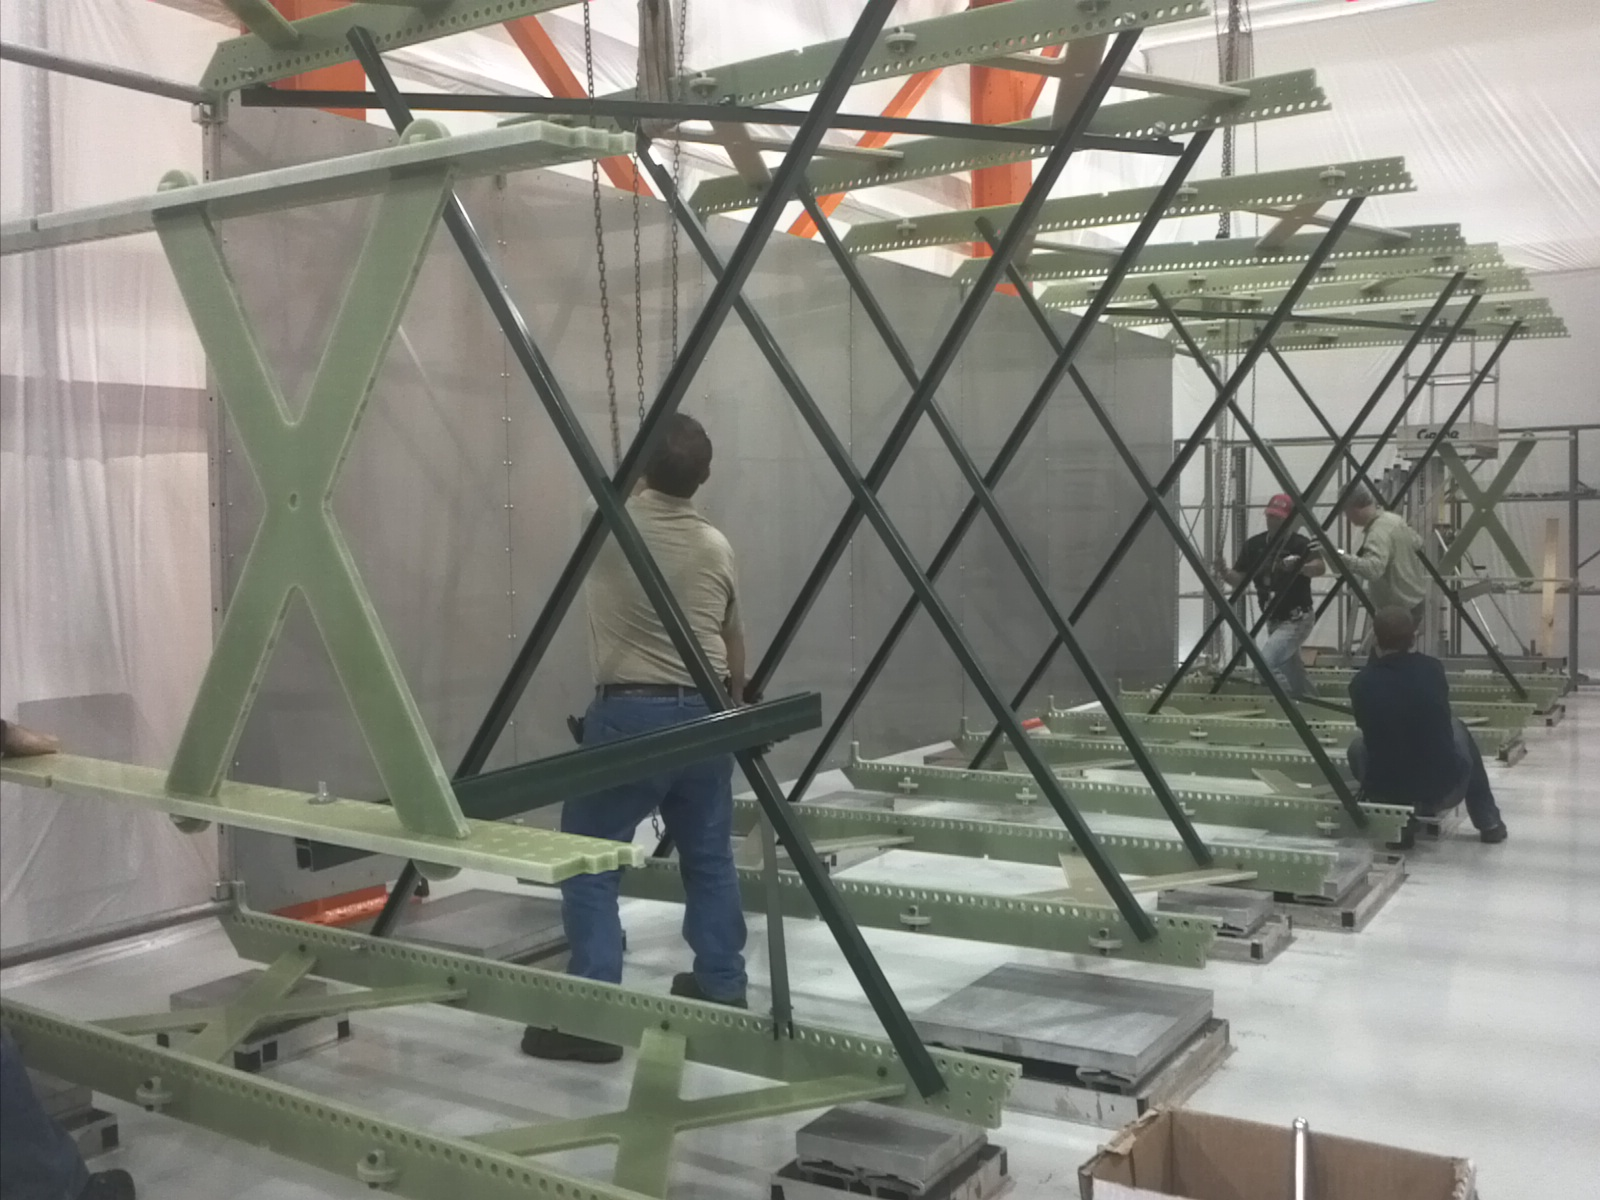
\includegraphics[width=0.7\linewidth]{figures/tpc-cathode-g10-frame.jpg}
%\caption{Cathode frame and G-10 ribs on metal assembly platforms.}
%\label{fig:tpc-cathode-g10-frame}
%\end{figure}

\subsubsection{Wire installation and tension measurements}
%{\it{Jonathan (and Ryan?)}}
During detector assembly the completed wire carrier assemblies (consisting of wires and supporting carrier boards on either end) were manually installed onto the adjustable tensioning bars residing in the C-channel of the supporting anode frame.  A team of two people installed each assembly onto the anode frame.  The collection plane was the first installed, followed by the middle induction plane, and then finally the inner induction plane.  Once all three anode planes were completely installed, the tensioning bars were adjusted and a survey was taken of the tension of all anode wires.  Tension was set according to the design criteria that it be small enough to prevent wire breakage during cool down and large enough to limit the maximum wire sag due to gravity to under 0.5 mm for any 5m long U or V wire.   Tension was measured via measuring the resonant frequency of a laser beam reflected from a plucked wire and incident on a photodiode connected to a spectrum analyzer program \cite{SpectrumLaboratory}.  The tension measuring equipment was developed and produced by the University of Wisconsin Physical Sciences Laboratory.  The tensioning bars were adjusted iteratively until the surveyed tension of all wires was within a range, approximately $\pm$1.0 N of the nominal value of 6.9 N, where no single wire was too taught or loose to create detector performance issues.  Figure \ref{fig:heatmap} shows the final surveyed tension of the wires for each plane.

\begin{figure}
\centering
%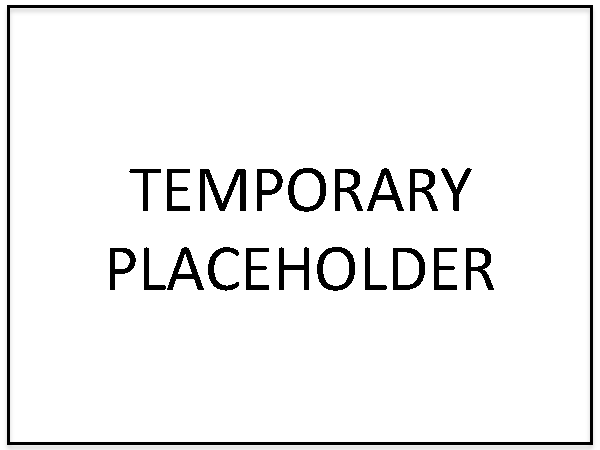
\includegraphics[width=2in]{figures/temp.pdf}
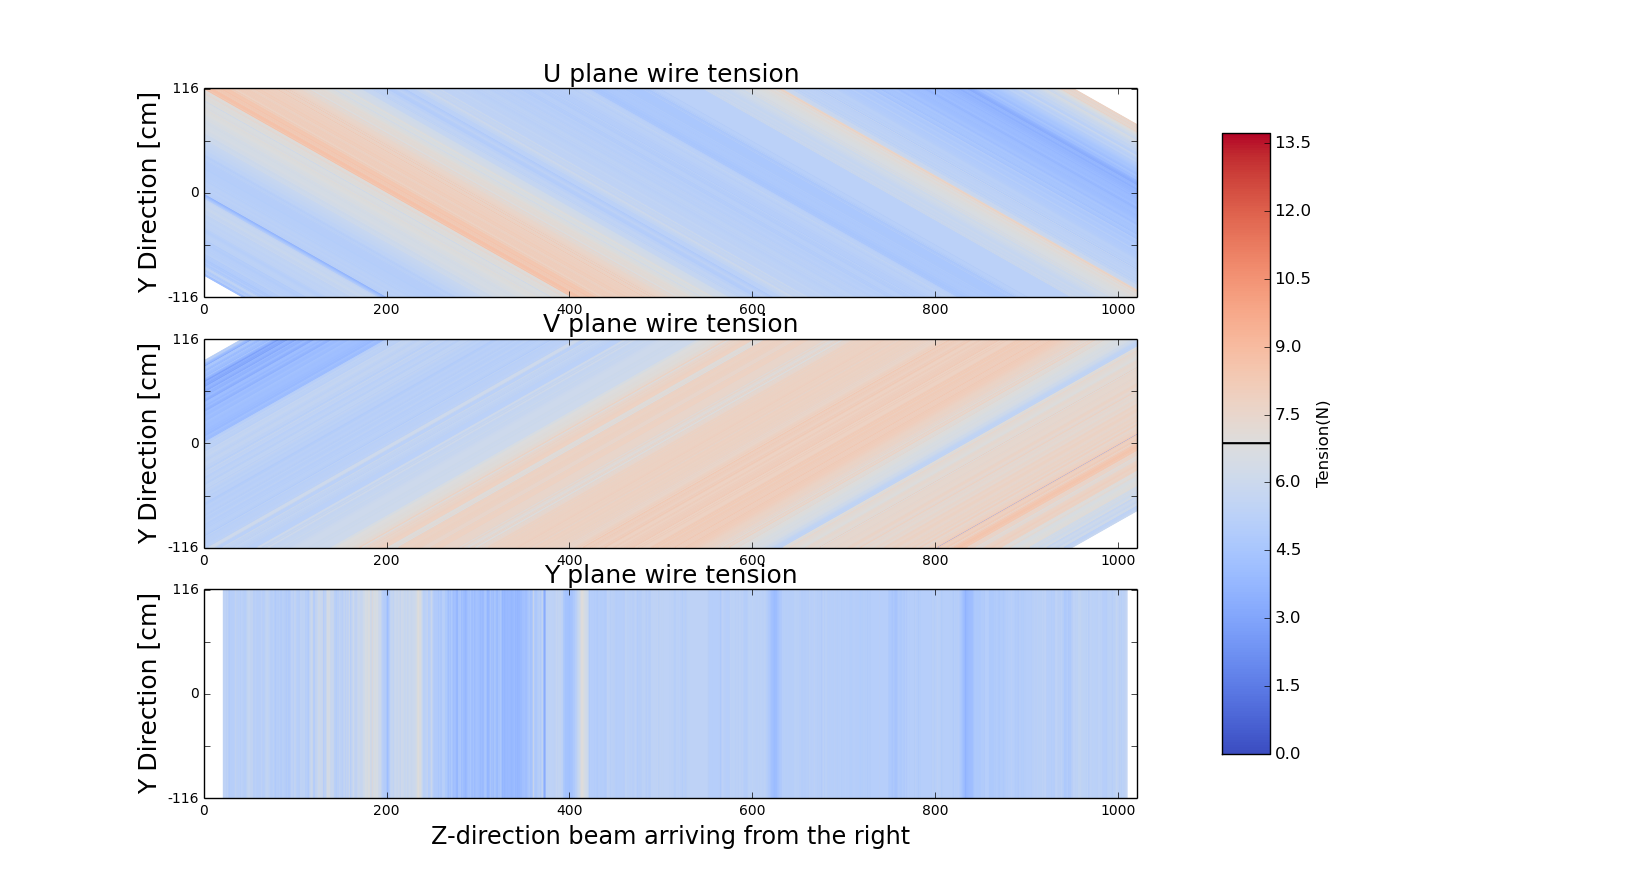
\includegraphics[width=0.95\textwidth]{figures/WireTension_201605_updatedcolors.png}
\caption{Final survey results for wire tension of the MicroBooNE LArTPC. All wires fall within the design wire tension specification of 6.9N $\pm$ 1.0N.}
\label{fig:heatmap}
\end{figure} 





%\input{tpc-hv}
\subsection{High Voltage System}
\label{sec:hv}
%{\it{Sarah, Cat}}

To create the drift field, negative voltage (referred to as the ``high-voltage'' or ``HV'') is supplied to the \lartpc cathode.  This potential is generated outside of the cryostat by a Glassman LX150N12 power supply.  Before entering the cryostat, the output of the power supply is passed through a current-limiting resistor chain that serves as both a low-pass filter for the power supply ripple, and a partition for the stored energy in the system.  The resistor chain is a set of eight 10 M$\Omega$ resistors connected in series and submerged in a transformer oil in an aluminum container.  This assembly was successfully tested to -200~kV. 

The potential is introduced into the cryostat by a custom-designed HV feedthrough.  The feedthrough is based on an ICARUS design~\cite{Amerio:2004-T600}; a 2.54 cm diameter stainless steel inner conductor is surrounded by a 5.08 cm outer diameter ultra-high molecular weight polyethylene (UHMW PE) tube that is encased in an outer ground tube.  A photograph and drawing of the production feedthrough are shown in figure~\ref{fig:hv_ftpic}.

% The label/referencing is terrible here because
% JINST does not like subfigures
\begin{figure}
\centering{
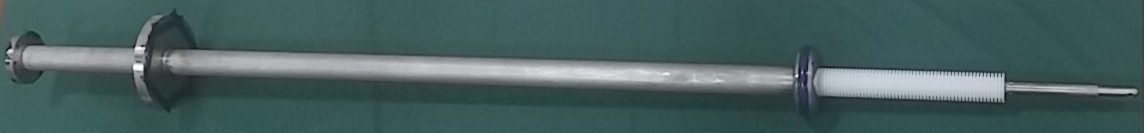
\includegraphics[width=\textwidth]{figures/hv-feedthrough}\\
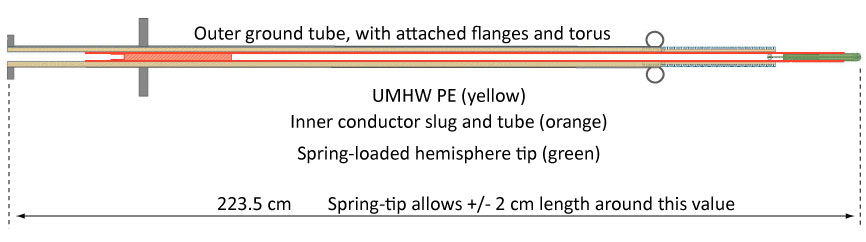
\includegraphics[width=\textwidth]{figures/hv-ftdrawing.jpg}
}
\caption{Photograph and drawing of the production HV feedthrough. The spherical probe tip is attached to the end of the inner conductor, on the right side of these figures.}
\label{fig:hv_ftpic}
\end{figure}

%The MicroBooNE TPC is a rectangular box resting inside of a cylindrical cryostat. Due to this geometry, the HV feedthrough must extend relatively deep into the cryostat in order to avoid high electric fields. Figure~\ref{fig:hv-FT-cryostat} shows the HV feedthrough extending into its receptacle cup, which is attached to the TPC cathode.  The lower termination of the outer ground tube is a torus chosen to minimize the electric field between the feedthrough and the nearby cathode plane and also along the feedthrough itself.  The length of exposed UHMW PE was machined with grooves with to reduce surface currents.  The electrical connection to the cathode is accomplished by way of a hemispherical spring-loaded tip attached to the inner conductor of the feedthrough; the tip makes contact with the receptacle cup attached to the cathode.

%MicroBooNE's voltage target combined with its geometry of a cylindrical cryostat with a single drift region necessitate that the HV feedthrough extend deeper into the cryostat than the ICARUS feedthrough to avoid high field regions.  
Figure~\ref{fig:hv-FT-cryostat} shows the HV feedthrough extending into its receptacle cup attached to the LArTPC cathode.  The lower termination of the outer ground tube is a torus chosen to reduce the electric field between both the feedthrough and the cathode plane, and along the feedthrough itself.  The electrical connection to the cathode is made with a hemispherical spring-loaded tip attached to the inner conductor of the feedthrough.  The UHMW PE tube is machined with grooves and extends into the receptacle cup attached to the cathode.

\begin{figure}
\centering{
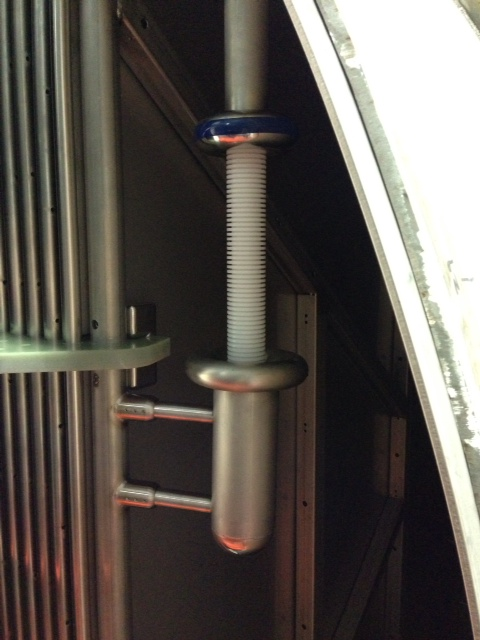
\includegraphics[width=0.6\textwidth]{figures/hv-FT-cryostat}
}
\caption{The production HV feedthrough inserted into the cathode receptacle cup inside the cryostat.}
\label{fig:hv-FT-cryostat}
\end{figure}
